\documentclass{mynote}




\graphicspath{{figures/}}
\title{大二下笔记合集}
\author{乐绎华}
\date{\today}


\begin{document}

\chapter{Main Content}

\tableofcontents


% Main includes directory
\input{includes/Appendix.tex}
\section{cmc 决赛备考}

\begin{enumerate}
	\item \textbf{优先采用教材上提供的基本方法和自然的思路.}
	\item \textbf{换序问题在时间比较富裕的情况下一定要严格证明.}
	\item \textbf{中值定理一定是自然的构造, 不要想的奇奇怪怪.}
	\item \textbf{填空题是基本盘, 一定不能错, 多检查, 可以猜答案.}
	\item \textbf{遇事不绝, 分部积分.}
	\item \textbf{遇事不绝, 不妨设标准型.}
	\item \textbf{数学类高年级组误判率较高! \underline{重代数轻分析}!}
	\item \textbf{第一天考完下午和晚上是最好玩的, 抓紧时机面基各路大神, 笔者当初考完带着一堆小伙伴去撸串, 干了十瓶可乐.}
	\item \textbf{考完当天晚上就会出成绩, 误判几率不低, 可以尽力配合老师查分.}
\end{enumerate}

\section{线性代数}

\begin{itemize}
	\item Jordan 分解
	\item 同时(正交)相似上三角/对角化\footnote{正交性要求特征值全为实数,或者实对称...}
	\item 两个半正定矩阵 $A,B$ 可以同时合同对角化.
	\item 实对称矩阵和正定矩阵显然可以同时合同对角化
	\item 矩阵打洞
	\item 摄动法,可以不妨设可逆
	\item $AB$ 和 $BA$ 有完全一样的非零 Jordan 块
	\item 与所有可逆矩阵可交换的矩阵是数量矩阵 $\lambda I$.
	\item 对 $A\in \mathbb{R}^{m\times n}$,有 $r(A^{T}A)=r(A)$.
	\item $r(A)=\dim \mathrm{Im}A=n-\dim \ker A$.
	\item $A$ 是半正定矩阵,等价于 $A$ 所有主子式\footnote{主子式是指取任意行和对应的列交叉出来的子式的行列式,代数主子式还要考虑逆序数.}非负,等价于 $A$ 的所有特征值为非负实数,等价于存在 $C\in \mathbb{R}^{n\times n}$ 使得 $A=C^{T}C$.
	\item 若 $A$ 可逆,则 $A^{-1}$ 是 $A$ 的多项式. 考虑特征多项式和哈密顿凯莱定理 (结合 $a_0\neq0$)
	\item $A^{*}$ 是 $A$ 的多项式. 注意到 $A^{*}=\lvert A \rvert A^{-1}$.
	\item 瑞丽商
	\item 反对称实矩阵的特征值实部为 0.
	\item 循环行列式
	\item 求解 $AX-XB=C$. 有唯一解的充要条件是 $A,B$ 无相同特征值. 证明考虑分块 Jordan 爆算. 这也是对于 $AX=XB$ 交结数的证明.
	\item 特征多项式等于极小多项式的等价条件.
	\item 覆盖定理
	\item 实正规矩阵\footnote{$AA^{T}=A^{T}A$}的正交相似标准型.
	\item 相似的正规矩阵必然酉相似. 若为实正规,则正交相似.
	\item 酉相似\underline{实}矩阵必然实正交相似.
	\item $A$ 是复正规矩阵的充要条件是 $A$ 的共轭转置是 $A$ 的多项式
	\item 三对角矩阵的行列式递推
	\item Perron 判别法
\end{itemize}

\begin{figure}[H]
\centering
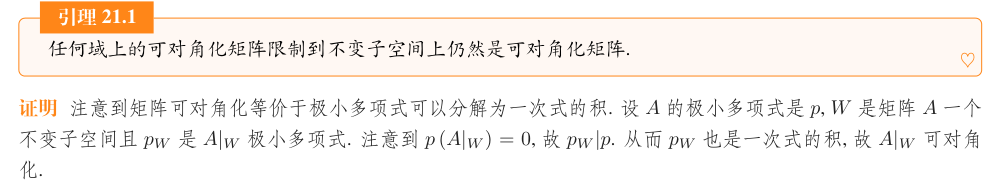
\includegraphics[width=\textwidth]{cmc决赛-2025040617.png}
% \caption{}
\label{}
\end{figure}
\begin{figure}[H]
\centering
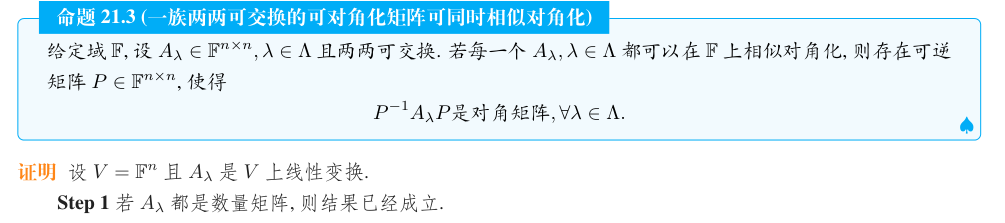
\includegraphics[width=\textwidth]{1-cmc决赛-2025040617.png}
% \caption{}
\label{}
\end{figure}
\begin{figure}[H]
\centering
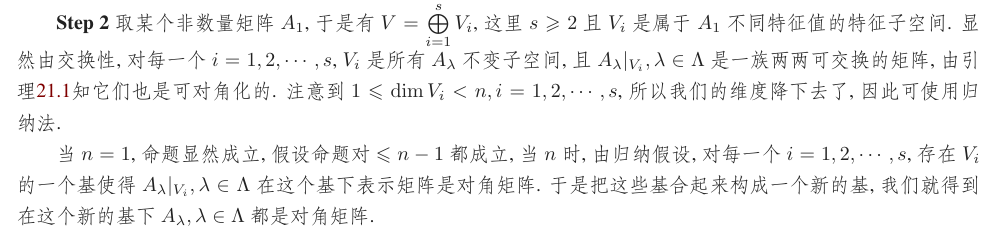
\includegraphics[width=\textwidth]{2-cmc决赛-2025040617.png}
% \caption{}
\label{}
\end{figure}
\begin{figure}[H]
\centering
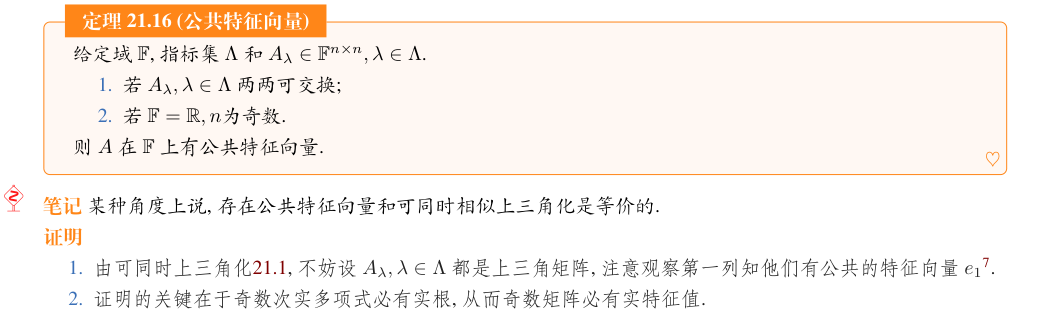
\includegraphics[width=\textwidth]{3-cmc决赛-2025040617.png}
% \caption{}
\label{}
\end{figure}
\begin{figure}[H]
\centering
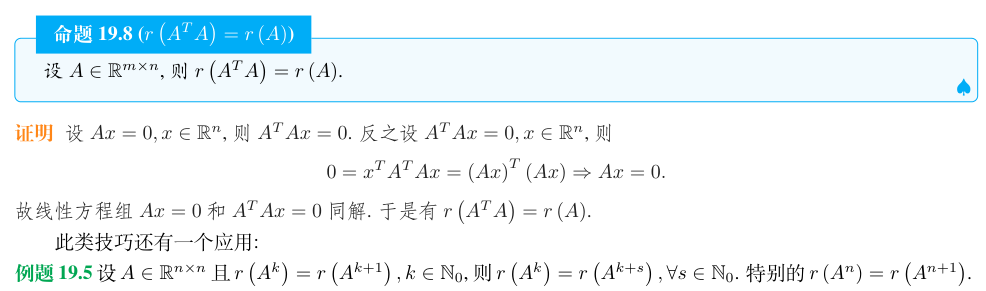
\includegraphics[width=\textwidth]{3-cmc决赛-2025040618.png}
% \caption{}
\label{}
\end{figure}
\begin{figure}[H]
\centering
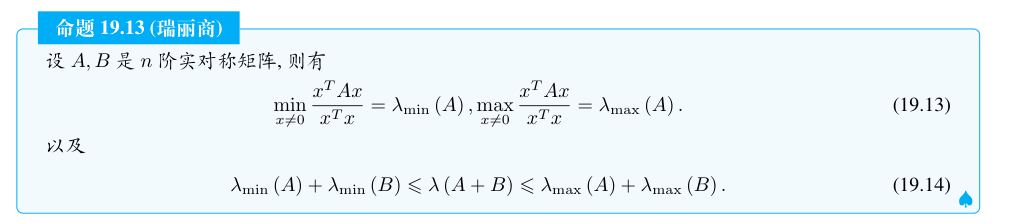
\includegraphics[width=\textwidth]{4-cmc决赛-2025040618.png}
% \caption{}
\label{}
\end{figure}
\begin{figure}[H]
\centering
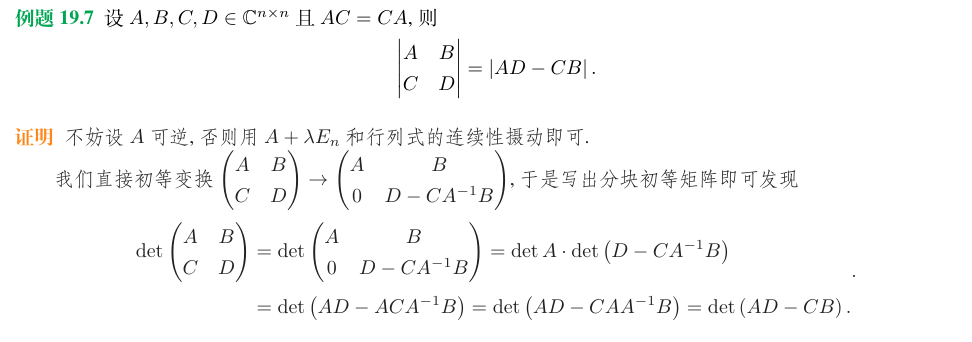
\includegraphics[width=\textwidth]{5-cmc决赛-2025040618.png}
% \caption{}
\label{}
\end{figure}
\begin{figure}[H]
\centering
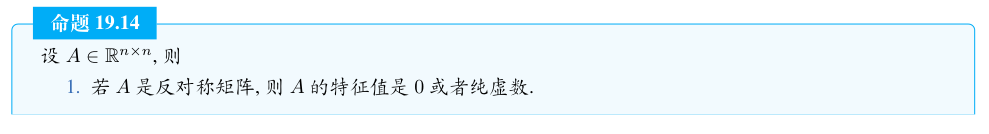
\includegraphics[width=\textwidth]{6-cmc决赛-2025040618.png}
% \caption{}
\label{}
\end{figure}
\begin{figure}[H]
\centering
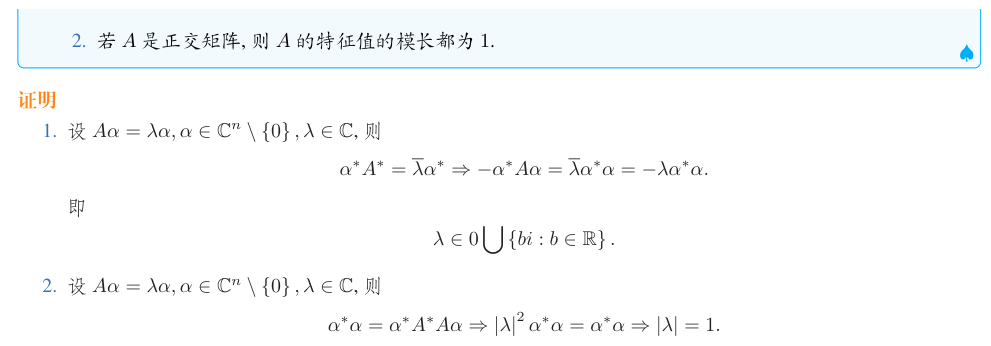
\includegraphics[width=\textwidth]{7-cmc决赛-2025040618.png}
% \caption{}
\label{}
\end{figure}
\begin{figure}[H]
\centering
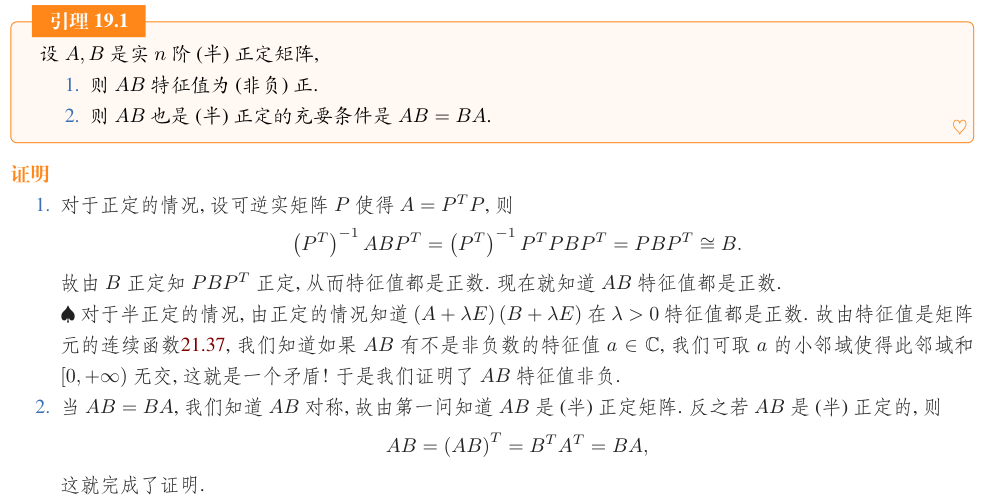
\includegraphics[width=\textwidth]{8-cmc决赛-2025040618.png}
% \caption{}
\label{}
\end{figure}
\begin{figure}[H]
\centering
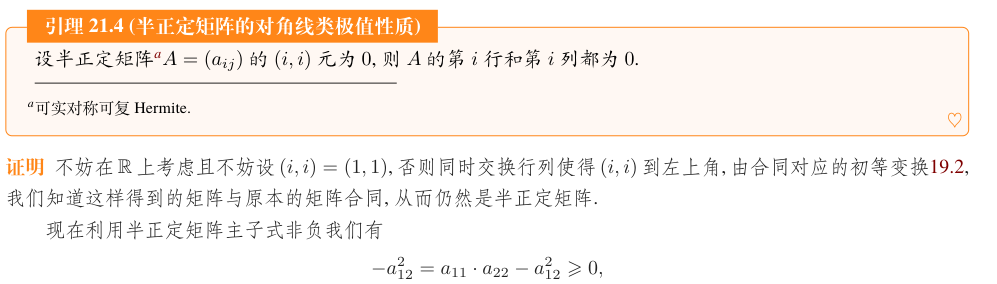
\includegraphics[width=\textwidth]{9-cmc决赛-2025040618.png}
% \caption{}
\label{}
\end{figure}
\begin{figure}[H]
\centering
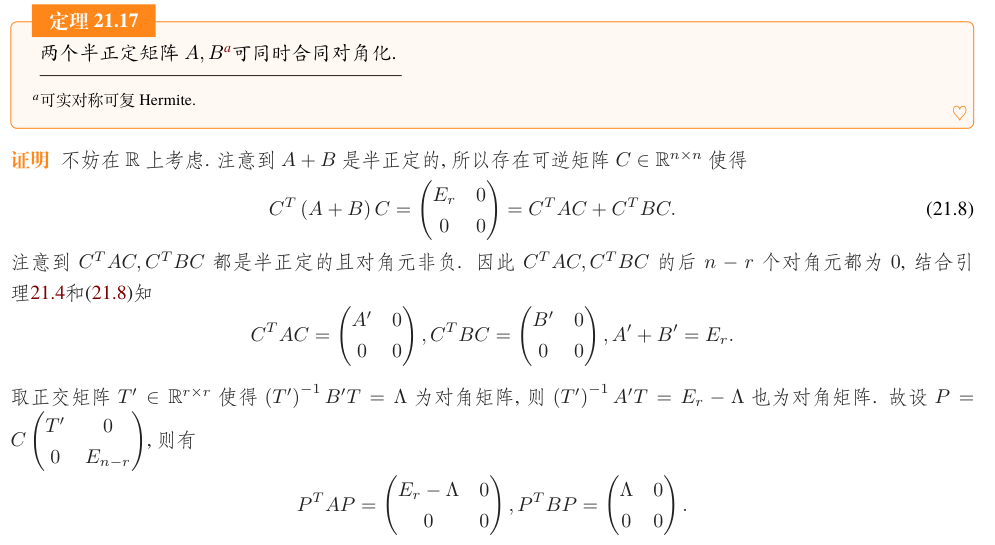
\includegraphics[width=\textwidth]{10-cmc决赛-2025040618.png}
% \caption{}
\label{}
\end{figure}
\begin{figure}[H]
\centering
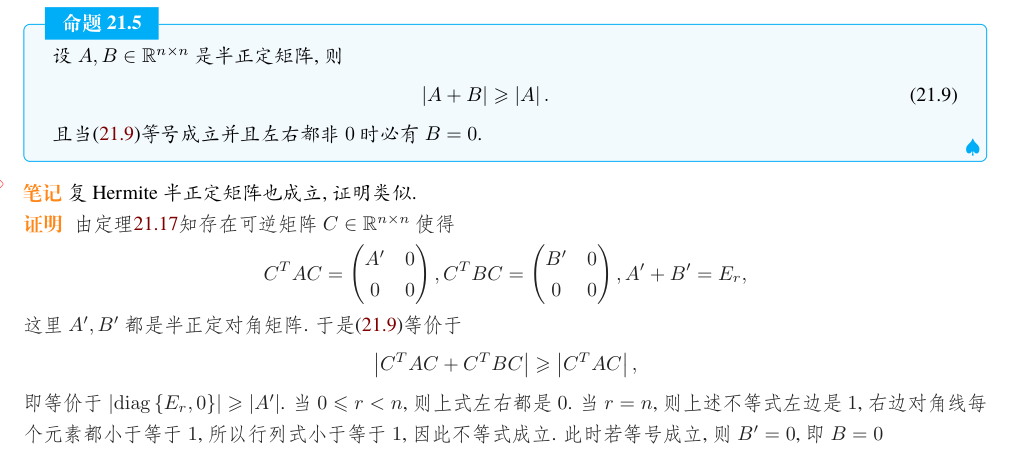
\includegraphics[width=\textwidth]{11-cmc决赛-2025040618.png}
% \caption{}
\label{}
\end{figure}
\begin{figure}[H]
\centering
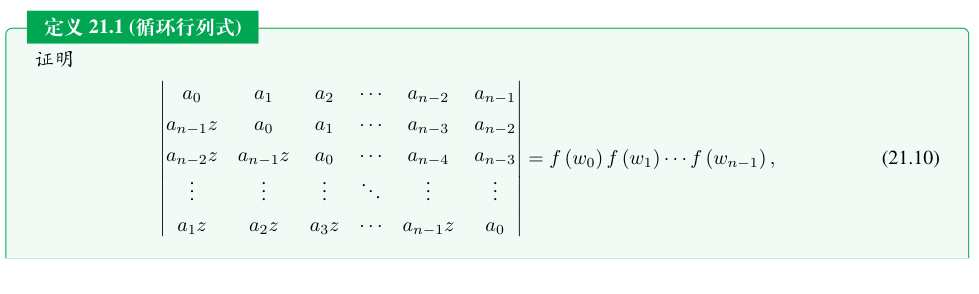
\includegraphics[width=\textwidth]{12-cmc决赛-2025040618.png}
% \caption{}
\label{}
\end{figure}
\begin{figure}[H]
\centering
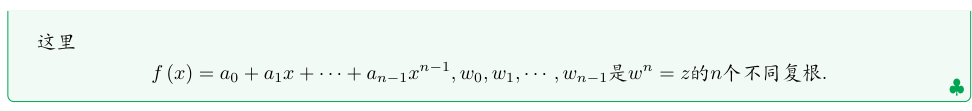
\includegraphics[width=\textwidth]{13-cmc决赛-2025040618.png}
% \caption{}
\label{}
\end{figure}
\begin{figure}[H]
\centering
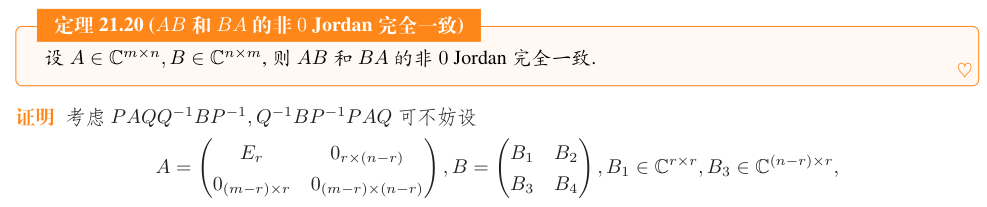
\includegraphics[width=\textwidth]{14-cmc决赛-2025040618.png}
% \caption{}
\label{}
\end{figure}
\begin{figure}[H]
\centering
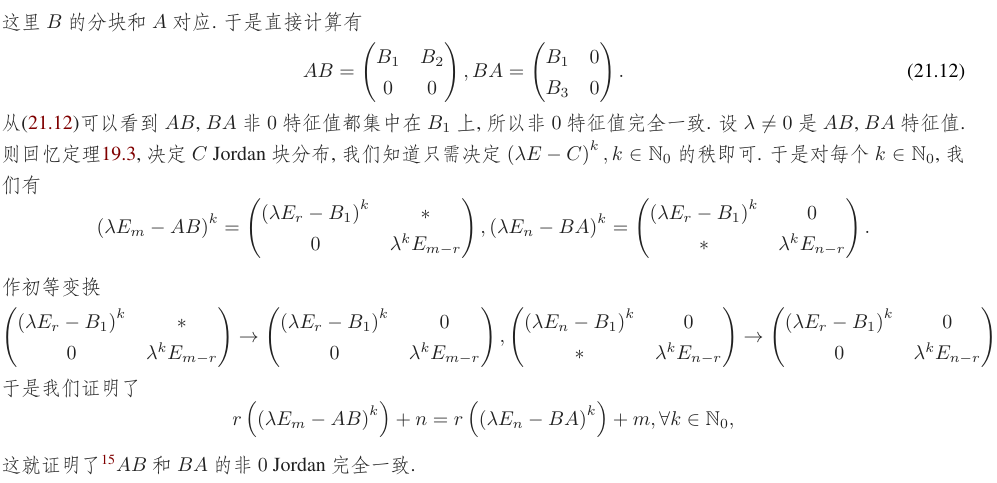
\includegraphics[width=\textwidth]{15-cmc决赛-2025040618.png}
% \caption{}
\label{}
\end{figure}

\begin{figure}[H]
\centering
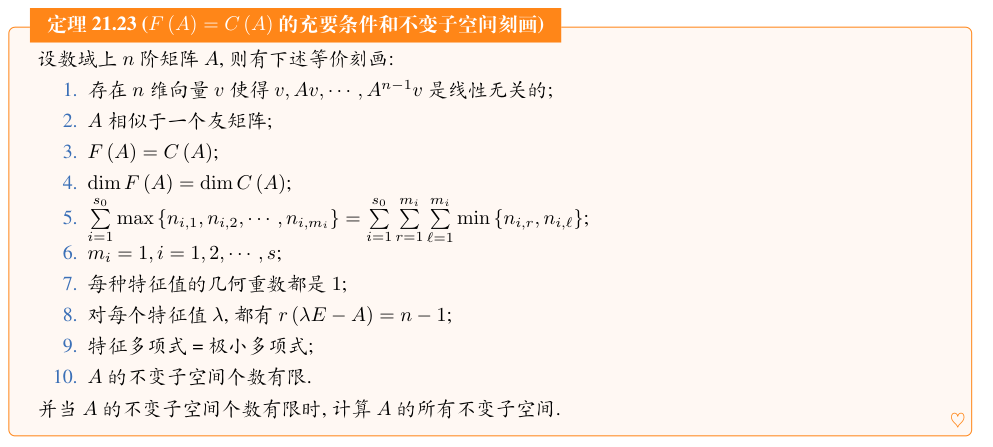
\includegraphics[width=\textwidth]{16-cmc决赛-2025040618.png}
% \caption{}
\label{}
\end{figure}
\begin{figure}[H]
\centering
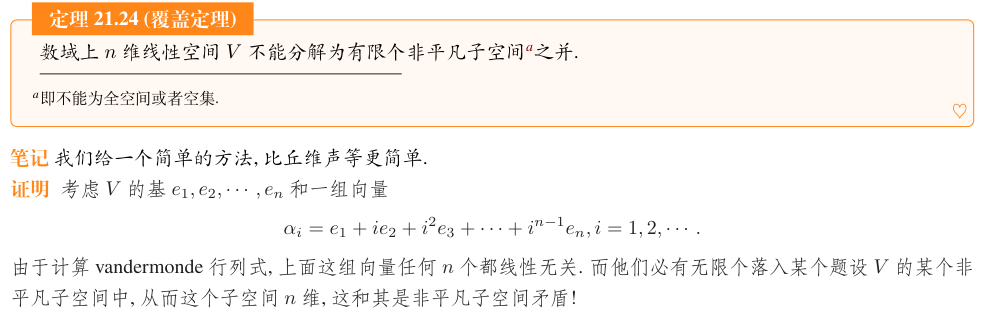
\includegraphics[width=\textwidth]{17-cmc决赛-2025040618.png}
% \caption{}
\label{}
\end{figure}
\begin{figure}[H]
\centering
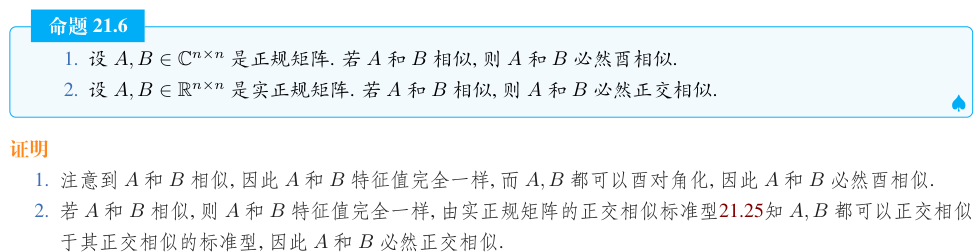
\includegraphics[width=\textwidth]{18-cmc决赛-2025040618.png}
% \caption{}
\label{}
\end{figure}

\section{数学分析}

\subsection{利用 \texorpdfstring{$\delta \epsilon$}{delta epsilon}}


\begin{theorem}
    若$f$在$[1,+\infty)$一致连续且广义可积,则$\lim_{n\to \infty}f(x)=0$.
\end{theorem}

\begin{note}
    $f$的一致连续性是必要的,反例见汪林数分反例第4章最后一个.
\end{note}

\begin{proof}
    $\forall \epsilon>0,\exists \delta>0,s.t.\forall x,y\in [1,+\infty),\left|x-y\right|<\delta\Rightarrow \left|f(x)-f(y)\right|<\epsilon.$ $\exists M>0,s.t.\forall x>M,\left|\int_{x}^{x+\delta}f(x)dx\right|<\textcolor{blue}{\delta\epsilon}.$Then
    $$\delta \left|f(x)\right|\le  \left|\int_{x}^{x+\delta}f(x)dt\right|\le \left|\int_{x}^{x+\delta}f(t)dt\right|+\delta \epsilon\le 2\delta \epsilon\Rightarrow \left|f(x)\right|\le 2\epsilon\Rightarrow \lim_{x\to \infty}f(x)=0.$$
\end{proof}

\begin{note}
    相同的证明思想,利用$\delta \epsilon$,同样出现在$f\in \mathscr{R}[a,b],g\in C[\inf f,\sup f]\Rightarrow g\circ f\in \mathscr{R}[a,b]$中.
\end{note}

\begin{theorem}\label{memeda22}
    $f\in \mathscr{R}[a,b],g\in C[\inf f,\sup f]\Rightarrow g\circ f\in \mathscr{R}[a,b]$
\end{theorem}

\begin{proof}
    $g\in C[a,b]\Rightarrow \forall \epsilon>0,\exists \delta>0,s.t.\forall x,y\in [a,b],\left|x-y\right|<\delta\Rightarrow \left|f(x)-f(y)\right|<\epsilon.$
    \\
    $\displaystyle \exists P=\{x_0,\cdots,x_n\}\ on\ [a,b], \sum_{i=0}^{n}(\sup_{[x_{i-1},x_i]}f-\inf_{[x_{i-1},x_{i}]}f)(x_i-x_{i-1})<\textcolor{blue}{\delta \epsilon}$. Then
    \begin{align*}
        \delta \epsilon
        &\ge \sum_{\left| f\left( x_{i-1} \right) -f\left( x_i \right) \right|\ge \delta}{\left( \underset{\left[ x_{i-1},x_i \right]}{\mathrm{sup}} f-\underset{\left[ x_{i-1},x_i \right]}{\mathrm{inf}} f \right)\left( x_i-x_{i-1} \right)}\\
        &\ge \delta \sum_{\left| f\left( x_{i-1} \right) -f\left( x_i \right) \right|\ge \delta}{\left( x_i-x_{i-1} \right)}\\
        &\Rightarrow \sum_{\left| f\left( x_{i-1} \right) -f\left( x_i \right) \right|\ge \delta}{\left( x_i-x_{i-1} \right)}\le \epsilon
    \end{align*}
    \begin{align*}
        &\sum_{i=0}^{n}\left(\sup_{[x_{i-1},x_i]}g\circ f-\inf_{[x_{i-1},x_{i}]}g\circ f\right)(x_i-x_{i-1})\\
        &\le \sum_{\left| f\left( x_{i-1} \right) -f\left( x_i \right) \right|<\delta}+\sum_{\left| f\left( x_{i-1} \right) -f\left( x_i \right) \right|\ge \delta}{\left( \underset{\left[ x_{i-1},x_i \right]}{\mathrm{sup}}g\circ f-\underset{\left[ x_{i-1},x_i \right]}{\mathrm{inf}}g\circ f \right)\left( x_i-x_{i-1} \right)} \\
        &\le (b-a)\epsilon +2\sup_{[x_{i-1},x_i]} \left|g\right|\epsilon
    \end{align*}
    Hence, $g\circ f\in \mathscr{R}[a,b]$.
\end{proof}

\begin{note}
    $f\in \mathscr{R}[a,b],g\in C[\inf f,\sup f]\nRightarrow f\circ g\in \mathscr{R}[a,b]$. 反例考虑$g$将正测集映到$f$的间断点集合(一个零测集),使得$g\circ f$的间断点集合是正测集,故$f\circ g\notin \mathscr{R}[a,b]$. 只需加强$g$的连续性使得零测集的原像都是零测集.
\end{note}

\subsection{利用单调性两边夹住}

\begin{exercise}
设 $f$ 在 $[0,+\infty)$ 上递增, 对于任何 $T>0, f$ 在 $[0, T]$ 上可积, 且
\begin{align*}
    \lim _{x \rightarrow+\infty} \frac{1}{x} \int_0^x f(t) d t=C .
\end{align*}

证明
\begin{align*}
    \lim _{x \rightarrow+\infty} f(x)=C .
\end{align*}
\end{exercise}

\begin{proof}
    $$\frac{\int_{0}^{x}f(t)dt}{x}\le f(x)\le \frac{\int_{x}^{2x}f(t)dt}{x}=\textcolor{blue}{\frac{\int_{0}^{2x}f(t)dt-\int_{0}^{x}f(t)dt}{x}}$$
    两边取$x\to \infty$得
    $$C\le \lim_{x\to \infty}f(x)\le 2C-C=C\Rightarrow f(x)=C$$
\end{proof}

\begin{exercise}
$f$在$[0,a)$单调,瑕积分$\int_{0}^{a}x^pf(x)dx$收敛,则$\lim_{x\to 0^+}x^{p+1}f(x)=0$.
\end{exercise}

\begin{proof}
    若$p=-1$,则显然$\lim_{x\to 0^+}x^{p+1}f(x)=0$,否则$\int_{0}^{a}x^pf(x)dx$不收敛. 若$p>-1$,不妨设$f$递减,则$\lim_{x\to 0^+}x^pf(x)=+\infty$.
    \begin{align*}
        \int_{0}^{x}t^pf(t)dt\ge \int_{0}^{x}t^pf(x)dt= \frac{1}{p+1}x^{p+1}f(x)\ge \textcolor{blue}{\int_{x}^{2x}t^pf(t)dt}
    \end{align*}
    由柯西收敛,令$x\to 0^+$得
    \begin{align*}
        0\ge\lim_{x\to 0^+}\frac{1}{p+1}x^{p+1}f(x)\ge 0\Rightarrow \lim_{x\to 0^+}\frac{1}{p+1}x^{p+1}f(x)=0.
    \end{align*}
\end{proof}

\begin{exercise}
若$a_n$递减,$\sum_{n=1}^{\infty}a_n$收敛,证明:$\lim_{n\to \infty}na_n=0$
\end{exercise}

\begin{proof}
    \begin{align*}
        0\le na_{2n} \le \textcolor{blue}{\sum_{k=n+1}^{2n}a_k}\to 0(\ as \ n\to \infty) \implies \lim_{n\to \infty}na_n=0
    \end{align*}
\end{proof}

\begin{note}
    注意这里还要补充$a_{2n+1}$这种奇数项的细节. $\lim_{n\to \infty}a_n=0$说明这是显然的.
\end{note}

\subsection{先后取极限}

\begin{exercise}[类似大O Tauber定理]
设$f$在$[a,+\infty)$上恒正,在任意有限区间$[a,b]$可积,且存在常数$M>0$,使得$\int_{a}^{+\infty}f(x)e^{-tx}dx\le M$. 则有$\int_{a}^{+\infty}f(x)dx$收敛.
\end{exercise}

\begin{proof}
    $\forall A>a,$
    \begin{align*}
        M &\ge \int_{a}^{A}f(x)e^{-tx}dx \ge \int_{a}^{A}f(x)(1-tx)dx\\
        &= \int_{a}^{A}f(x)dx-t\int_{a}^{A}xf(x)dx\\
        &\to \int_{a}^{A}f(x)dx\ (as\ t\to 0^+)
    \end{align*}
    因此 $\int_{a}^{+\infty}f(x)dx\le M$. 由单调有界可知$\int_{a}^{+\infty}f(x)dx$收敛.
\end{proof}

\begin{note}
    下面几个定理见《阶的估计基础》chap6
\end{note}

\begin{theorem}[大O Tauber定理]
    \footnote{这是定理\cref{memeda1}的推论}设
    \begin{align*}
        \begin{gathered}
            f(x)=O\left(\frac{1}{x}\right), \\
            F(x)=\int_0^{\infty} e^{-x t} f(t) d t \rightarrow s, \quad x \rightarrow 0+.
        \end{gathered}
    \end{align*}

    则必有
    \begin{align*}
        \int_0^{\infty} f(t) d t=s
    \end{align*}
\end{theorem}

\begin{theorem}
    设 $f(x)$ 为 $(0, \infty)$ 内的非负函数,
    \begin{align*}
        F(x)=\int_0^{\infty} e^{-x t} f(t) d t, \quad x>0 .
    \end{align*}

    若
    \begin{align*}
        F(x) \sim \frac{s}{x^\alpha}, \quad \alpha>0, x \rightarrow 0+
    \end{align*}
    则必有
    \begin{align*}
        \int_0^x f(t) d t \sim \frac{s x^\alpha}{\Gamma(\alpha+1)}, \quad x \rightarrow \infty .
    \end{align*}
\end{theorem}

\begin{corollary}
    设
    \begin{align*}
        a_n \geq 0, \quad \sum_{n=0}^{\infty} a_n x^n \sim \frac{s}{1-x}, \quad x \rightarrow 1-.
    \end{align*}

    则
    \begin{align*}
        \sum_{k=0}^n a_k \sim s n, \quad n \rightarrow \infty .
    \end{align*}
\end{corollary}

\begin{theorem}\label{memeda1}
    设
    \begin{align*}
        \begin{gathered}
            f(x)>-\frac{B}{x}, \quad 0<x<\infty, \\
            F(x)=\int_0^{\infty} e^{-x t} f(t) d t \rightarrow s, \quad x \rightarrow 0+.
        \end{gathered}
    \end{align*}

    则
    \begin{align*}
        \int_0^{\infty} f(t) d t=s .
    \end{align*}
\end{theorem}

\subsection{利用额外的参量}

\begin{exercise}
设 $0 \leqslant a<b$, 是否存在 $f \in C[a, b]$ 使得
$$
    \int_a^b f(x) x^{2 n} \mathrm{~d} x>0, \int_a^b f(x) x^{2 n+1} \mathrm{~d} x<0, n=0,1,2, \cdots .(*)
$$

如果存在, 请给出存在, 如果不存在, 请给出理由.
\end{exercise}

\begin{proof}
    我们考虑 $F(t)=\int_a^b f(x) e^{-x t} d x, \textcolor{blue}{t} \geqslant 0$, 则容易得到
    $$
        |F(t)| \leqslant \max _{[a, b]}|f| \cdot \int_0^{\infty} e^{-x t} d x=\frac{\max _{[a, b]}|f|}{t},
    $$

    即 $\lim _{t \rightarrow+\infty} F(t)=0$.

    但是对任何 $t>0$, 我们都有
    $$
        F(t)=\int_a^b f(x) e^{-x t} d x=\sum_{n=0}^{\infty} \int_a^b f(x) \frac{(-x t)^n}{n!} d x=\sum_{n=0}^{\infty} \frac{(-1)^n t^n}{n!} \int_a^b f(x) x^n d x \stackrel{(*)}{\geqslant} \int_a^b f(x) d x>0 .
    $$

    这就是一个矛盾! 因此我们证明了满足题目条件的 $f$ 不存在.
\end{proof}

\begin{exercise}[反向洛必达]
设 $f \in C[0,+\infty) \cap C^2(0,+\infty)$ 且 $f^{\prime \prime}(x)>-\frac{C}{x^2}$, 则有
$$
    \lim _{x \rightarrow 0^{+}} x f^{\prime}(x)=0 \text {. }
$$
\end{exercise}

\begin{proof}
    不妨设 $C>0$, 对 $h>0$, 由 Taylor 中值定理我们知道存在 $\theta \in(x, x+h)$, 使得
    $$
        f(x+h)=f(x)+f^{\prime}(x) h+\frac{f^{\prime \prime}(\theta)}{2} h^2 .
    $$

    于是
    $$
        f^{\prime}(x)=\frac{f(x+h)-f(x)}{h}-\frac{f^{\prime \prime}(\theta)}{2} h .
    $$

    于是运用条件就有
    $$
        f^{\prime}(x) \leqslant \frac{|f(x+h)-f(x)|}{h}+\frac{C}{2 \theta^2} h \leqslant \frac{|f(x+h)-f(x)|}{h}+\frac{C}{2 x^2} h .
    $$

    我们取 $\textcolor{blue}{h=\eta x, \eta \in(0,1)}$, 就有
    $$
        x f^{\prime}(x) \leqslant x \frac{|f(x+\eta x)-f(x)|}{\eta x}+x \frac{C}{2 x^2} \eta x=\frac{|f(x+\eta x)-f(x)|}{\eta}+\frac{C \eta}{2},
    $$

    因此就有
    $$
        \varlimsup_{x \rightarrow 0^{+}}\left[x f^{\prime}(x)\right] \leqslant \frac{C \eta}{2}
    $$

    由 $\eta$ 任意性可得
    $$
        \varlimsup_{x \rightarrow 0^{+}}\left[x f^{\prime}(x)\right] \leqslant 0 .
    $$

    类似的由 Taylor 中值定理我们知道存在 $\vartheta \in(x-h, x)$, 使得
    $$
        f(x-\eta x)=f(x)-f^{\prime}(x) \eta x+\frac{f^{\prime \prime}(\vartheta)}{2} \eta^2 x^2 .
    $$

    于是
    $$
        \begin{aligned}
            x f^{\prime}(x) & =\frac{f(x)-f(x-\eta x)}{\eta}+\frac{f^{\prime \prime}(\vartheta)}{2} \eta x^2 \geqslant-\frac{|f(x)-f(x-\eta x)|}{\eta}-\frac{C}{2 \vartheta^2} \eta x^2 \\
                            & \geqslant-\frac{|f(x)-f(x-\eta x)|}{\eta}-\frac{C}{2(x-\eta x)^2} \eta x^2=-\frac{|f(x)-f(x-\eta x)|}{\eta}-\frac{C \eta}{2(1-\eta)^2},
        \end{aligned}
    $$

    于是
    $$
        \varliminf_{x \rightarrow 0^{+}}\left[x f^{\prime}(x)\right] \geqslant-\frac{C \eta}{2(1-\eta)^2} \text {. }
    $$

    由 $\eta$ 任意性可得
    $$
        \varliminf_{x \rightarrow 0^{+}}\left[x f^{\prime}(x)\right] \geqslant 0 .
    $$

    因此我们证明了
    $$
        \lim _{x \rightarrow 0^{+}}\left[x f^{\prime}(x)\right]=0 .
    $$
\end{proof}

\subsection{先后两次判断收敛}

\begin{theorem}
    数列$u_n,v_n$单调有界,$\lim_{n\to \infty}u_n=0$,证明:$\sum_{n=1}^{\infty}(-1)^{n-1}u_nv_n$收敛.
\end{theorem}

\begin{proof}
    由狄利克雷判别法:$\sum_{n=1}^{\infty}(-1)^{n-1}u_n$收敛,再由阿贝尔判别法:$\sum_{n=1}^{\infty}(-1)^{n-1}u_nv_n$收敛.
\end{proof}

\subsection{不同意义下的收敛}

\subsubsection{级数收敛}

\begin{definition}
    对于级数$\sum_{n=1}^{\infty}c_n$,记$s_k=\sum_{n=1}^{k}c_n.$
    \begin{itemize}
        \item 普通收敛:$$\lim_{k\to \infty}s_k \ exists$$
        \item Cesàro收敛:$$\lim_{N\to \infty}\sigma_N=\lim_{N\to \infty}\frac{s_1+s_2+\cdots+s_N}{N}\ exists $$
        \item Abel收敛:$$\lim_{r\to 1^-}A(r)=\lim_{r\to 1^-}\sum_{k=0}^{\infty}c_kr^k\ exists$$
    \end{itemize}
\end{definition}

三者的蕴含关系以及反例:

\begin{center}
    \begin{tikzcd}[row sep = tiny, column sep = tiny, font=\small]
        \text{普通收敛} \arrow[rr,Rightarrow,bend left] & \{(-1)^n\}_{n\ge 1} & \text{Cesàro收敛} \arrow[ll,Rightarrow,bend left,"/"{marking} ] \arrow[rr,Rightarrow,bend left] & \{(-1)^{n}n\}_{n\ge 1} & \text{Abel收敛} \arrow[ll,Rightarrow,bend left,"/"{marking} ]\\
        & & & & \\
        D_N(x)=\frac{\sin \left(\left(N+\frac{1}{2}\right) x\right)}{\sin (x / 2)} \arrow[uu,"D_N*f=S_N"description] & & F_N(x)=\frac{1}{N} \frac{\sin ^2(N x / 2)}{\sin ^2(x / 2)} \arrow[uu,"F_N*f=\sigma_N"description] & & P_r(\theta)=\frac{1-r^2}{1-2 r \cos \theta+r^2} \arrow[uu,"P_r*f=\lim_{r\to  1^-}A_f(r)"description]
    \end{tikzcd}
\end{center}

\begin{note}
    下面的级数$\sum_{n=1}^{\infty}c_n$有时代指$f$的傅里叶级数.
\end{note}

\begin{corollary}
    设 $\lim _{n \rightarrow \infty} \sum_{k=1}^n a_k$ 存在, 则
    \begin{align*}
        \lim _{n \rightarrow \infty} \frac{\displaystyle\sum_{k=1}^n k a_k}{n}=0 .
    \end{align*}
\end{corollary}

\begin{note}
    这题不能直接使用Stolz公式.
\end{note}

\begin{proof}
    \begin{align*}
        \lim _{n \rightarrow \infty} \frac{\displaystyle\sum_{k=1}^n k a_k}{n}
         & =
        \lim _{n \rightarrow \infty} \sum_{k=1}^n a_k-\frac{\displaystyle\sum_{k=1}^n (n-k) a_k}{n}   \\
         & =
        \lim _{n \rightarrow \infty} \sum_{k=1}^n a_k-\frac{\displaystyle\sum_{k=1}^n s_k}{n}         \\
         & =
        \lim _{n \rightarrow \infty}\sum_{k=1}^n a_k-\textcolor{blue}{\text{Cesaro mean of }}\sum a_k \\
         & =0                                                                                         \\
    \end{align*}
\end{proof}


\begin{theorem}
    $f$可积,若$f$在$x_0$处连续,则$\lim_{r\to 1^-}A_f(r)(x_0)=f(x_0)$. 若$f$在$x_0$处跳跃间断,则$\lim_{r\to 1^-}A_f(r)(x_0)=\frac{f(x_0^-)+f(x_0^+)}{2}$.
\end{theorem}

\begin{theorem}[Tauber's lemma]
    若$\sum c_n$有Abel收敛到$s$,且$c_n=o(1/n)$\footnote{在Littlewood的版本中,$c_n=O(1/n)$也对,见Stein傅里叶分析p63 exercise 3},则$\sum c_n$收敛到$s$. 即$\lim_{r\to 1^-}\sum c_nr^n=\sum c_n$.
\end{theorem}

\begin{note}
    这可以用来考察收敛半径为1的幂级数在收敛域边界上是否收敛. 若有$c_n=o(1/n)$,则收敛.
\end{note}

\begin{theorem}
    $f$可积,且$\hat{f}(\nu)=O(1/\left|\nu\right|)$,则若$f$在$\theta $连续,则$S_N(f)(\theta)\to f(\theta)\ (as\ N\to \infty)$,若跳跃间断,则$S_N(f)(\theta)\to \frac{f(\theta-)+f(\theta+)}{2}$. 若$f\in C[-\pi ,\pi ]$,则$S_N(f)\to f$ uniformly.
\end{theorem}

% \begin{theorem}[weak version of Littlewood's theorem]
%     $\sum c_n$有Cesaro收敛到$s$,且$c_n=O(1/n)$,则$\sum c_n$收敛到$s$. 
% \end{theorem}

\subsection{傅里叶变换的对称性}

$f$的光滑性与$\hat{f}$的阶:

\begin{center}
    \begin{tikzcd}[row sep = tiny, column sep = tiny, font=\tiny]
        f\in C^k \arrow[r,rightsquigarrow] & \hat{f}=o(1/\left|n\right|^k) & \text{integrate by parts and use Riemann-Lebesgue lemma}\\
        f\text{ is Lipschitz} \arrow[r,rightsquigarrow] & \hat{f}=o(1/\left|n\right|^k) & \text{使用事实\ref{factos}并分段估计}\\
        f\text{ is monotonic} \arrow[r,rightsquigarrow] & \hat{f}=O(1/\left|n\right|) & \text{使用简单函数逼近,或者在实数情况下使用第二积分中值定理}\\
        f\in BV \arrow[r,rightsquigarrow] & \hat{f}=O(1/\left|n\right|) & \text{强行构造分段使用积分第二积分中值定理}\\
        f\ \alpha-\text{Holder连续} \arrow[r,rightsquigarrow] & \hat{f}=O(1/\left|n\right|^\alpha) & \text{使用事实\ref{factos}并分段估计}\\
        f\text{ merely Riemann integrable} \arrow[r,rightsquigarrow] & \hat{f}=o(1) & \text{由Parseval恒等式:}\sum \left|\hat{f}\right|^2=\int_{\mathbb{R}}\left|f\right|^2<\infty\\
    \end{tikzcd}
\end{center}

\begin{property}[factos]\label{factos}
    \begin{align*}
        \hat{f}(n)=-\frac{1}{2 \pi} \int_{-\pi}^\pi f(x+\pi / n) e^{-i n x} d x
    \end{align*}
    hence
    \begin{align*}
        \hat{f}(n)=\frac{1}{4 \pi} \int_{-\pi}^\pi[f(x)-f(x+\pi / n)] e^{-i n x} d x .
    \end{align*}
\end{property}

\subsection{两种方式估阶,阶不同故矛盾}

\begin{note}
    见stein傅里叶分析p117关于Weierstrss函数处处连续但不可导的性质的讨论.
\end{note}

\subsection{反例}

对于$[1,+\infty)$上的正值连续函数$f$,$\sum_{n=1}^{\infty}f(n)$与$\int_{1}^{\infty}f(x)dx$的敛散性互不蕴含.

\begin{note}
    但是对于非负不增函数上面的敛散性是等价的. 这说明非负不增性不能被正值连续性替代. 反例见《实分析中的反例》p113.
\end{note}

级数$\sum_{n=1}^{\infty}a_n$收敛蕴含$\sum_{n=1}^{N}a_n\ (\forall N\in \mathbb{N})$有界且$\lim_{n\to \infty}a_n=0$. 但是反过来不对,有反例,见《实分析中的反例》p103.

级数收敛充要条件(柯西收敛准则)是$\lim_{m,n\to \infty}(a_{n+1}+\cdots+a_{m})=0$,这里$m,n$是无关的. 若$m,n$相关,即$\lim_{n\to \infty}(a_{n+1}+\cdots+a_{m(n)})=0$,则推不出来级数$\sum_{n=1}^{\infty}a_n$收敛,反例考虑调和级数$\sum 1/n$,具体见《实分析中的反例》p106.

% \begin{property}[factos]
%     $$
%     z=\text{Re}(z)-i\text{Re}{iz}
%     $$
% \end{property}

\subsection{隔开边界}

\begin{theorem}[解析函数序列收敛性]\label{ }
    一列调和函数$\displaystyle \{f_n\}_{n=1}^\infty$在 $\displaystyle \Omega$内的紧集上一致收敛到 $\displaystyle f$, 那么 $\displaystyle \{f'_n\}_{n=1}^\infty$在 $\displaystyle \Omega$内的紧集上一致收敛到 $\displaystyle f'$.
\end{theorem}

\begin{proof}
    不妨设 $\displaystyle \{f_n\}_{n=1}^\infty$在 $\displaystyle \Omega$上一致收敛到 $\displaystyle f$. 记$\Omega_\delta=\{z\in \Omega:\overline{D_\delta}(z)\in \Omega\}$. 断言对于$\Omega$内的解析函数$F$,有 $\displaystyle \sup_{z\in \Omega_\delta}\left|F'(z)\right|\leq \frac{1}{\delta}\sup_{\zeta\in \Omega}\left|F(\zeta)\right|$. 于是
    $$
        \sup_{x\in \Omega_\delta}\left|f'(z)-f'_n(z)\right|\leq \frac{1}{\delta}\sup_{\zeta\in \Omega}\left|f(z)-f_n(z)\right|\rightarrow 0(\text{ as }n\to \infty)\ \ \textcolor{blue}{\forall \delta>0}
    $$
    下面证明断言:
    \begin{align*}
        \left|F'(z)\right| & =\left|\frac{1}{2\pi i}\int_{C_\delta(z)} \frac{F(\zeta)}{(\zeta-z)^2 }d\zeta \right|             \\
                           & \leq \frac{1}{2\pi}\int_{C_\delta(z)} \frac{\left|F(\zeta)\right|}{\left|\zeta-z\right|^2 }d\zeta \\
                           & \leq \frac{1}{2\pi} \sup_{\zeta\in \Omega}\left|F(\zeta)\right| \frac{1}{\delta^2}2\pi \delta     \\
                           & =\frac{1}{\delta}\sup_{\zeta\in \Omega}\left|F(\zeta)\right|
    \end{align*}
\end{proof}

\subsection{广义黎曼引理}

\begin{note}
    注意到黎曼引理的证明并不依赖于$g$的周期性,只需要$\displaystyle \lim_{x\to +\infty}\frac{1}{x}\int_{0}^{x}g(t)dt$存在即可.
\end{note}

\begin{theorem}[广义黎曼引理]\label{广义黎曼引理}
    设$f(x)$在$[0,+\infty)$上绝对可积. 有界函数$g(x)$在任意区间上可积且$\displaystyle A=\lim_{x\to +\infty}\frac{1}{x}\int_{0}^{x}g(t)dt$存在,则
    \begin{align*}
        \lim_{\lambda\to \infty}\int_{0}^{\infty}f(x)g(\lambda x)dx=A\int_{0}^{\infty}f(x)dx
    \end{align*}
\end{theorem}

利用广义黎曼引理\cref{广义黎曼引理},我们可以解决下面问题:

\begin{exercise}
设 $f(x) \in C^1[0,+\infty)$, 已知 $\displaystyle \lim _{x \rightarrow+\infty} f(x)=0 、 f(0)=1$, 且 $f^{\prime}(x)$ 在 $[0,+\infty)$ 上绝对可积. 已知部分和有界的序列 $\left\{a_n\right\}(n \in \mathbb{N})$ 的 Cesaro 和为 $A$, 且满足对任意 $\displaystyle t>0, \sum_{n=0}^{\infty} a_n f(t n)$ 都收敛. 证明: $\displaystyle \lim _{t \rightarrow 0^{+}} \sum_{n=0}^{\infty} a_n f(t n)=A$.
\end{exercise}

\subsection{Wiener-Tauberian定理}

\begin{theorem}[Wiener-Tauberian定理]\label{ Wiener-Tauberian定理}
    设 $f(x)$ 是 $\mathbb{R}$ 上的绝对可积函数, 且 $f(x)$ 的 Fourier 变换没有零点,即
    $$
        \widehat{f}(x)=\frac{1}{\sqrt{2 \pi}} \int_{-\infty}^{+\infty} f(t) \mathrm{e}^{-\mathrm{i} x t} \mathrm{~d} t \neq 0, \quad x \in \mathbb{R} .
    $$

    若对于在任意区间上可积,且在 $\mathbb{R}$ 上有界的函数 $h(x)$ 有
    $$
        \lim _{x \rightarrow+\infty} \int_{-\infty}^{+\infty} h(x-t) f(t) \mathrm{d} t=A \int_{-\infty}^{+\infty} f(t) \mathrm{d} t \text {, }
    $$

    那么对任意在 $\mathbb{R}$ 上绝对可积函数 $g(x)$, 会有以下等式
    $$
        \lim _{x \rightarrow+\infty} \int_{-\infty}^{+\infty} h(x-t) g(t) \mathrm{d} t=A \int_{-\infty}^{+\infty} g(t) \mathrm{d} t .
    $$
\end{theorem}

\begin{note}
    这个定理可以用来证明Riemann-Lebesgue引理.
\end{note}

\begin{remark}
    提示: 建议考虑先证明 $\displaystyle \lim _{x \rightarrow+\infty} \int_0^1 \sin (x t) \mathrm{d} t=0$, 然后你会发现上述积分都形如 $\displaystyle F(x)=\int_0^{+\infty} f(t) h(x t) \mathrm{d} t$, 我们可以通过令 $x=\mathrm{e}^u , t=\mathrm{e}^{-s}$, 就可以得到卷积的形式.
\end{remark}

\subsection{求导证明是常数}

例如平均值公式的证明\cref{memeda14}, 例如《微分几何例题详解和习题汇编 by 陈维桓》p30.

\subsection{多项式插值}

\begin{theorem}
    若 $x_0, x_1, \cdots, x_n$ 是不同的实数, 则对任意数值 $y_0, y_1, \cdots, y_n$, 存在唯一的次数至多是 $n$ 次的多项式 $p_n$, 使得
    $$
        p_n\left(x_i\right)=y_i, 0 \leq i \leq n .
    $$
\end{theorem}

\begin{proof}
    唯一性:若$p_n,q_n$都是使得插值成立的至多是 $n$ 次的多项式,则
    \begin{align*}
        (p_n-q_n)(x_i)=0,\ 0\leq i\leq n.
    \end{align*}
    多项式$p_n-q_n$有$n+1$个零点,根据代数基本定理,$p_n-q_n$平凡,即$p_n=q_n$.

    存在性:考虑拉格朗日插值法,直接构造出来插值多项式.
\end{proof}

\begin{theorem}[插值多项式误差定理]\label{插值多项式误差定理}
    若$p(x)$是$f(x)$在点$x_0< x_1< \cdots< x_n$处的插值多项式,则
    \begin{align*}
        p(x)-f(x)=\frac{1}{(n+1)!}f^{(n+1)}(\xi_x)\prod_{i=0}^{n}(x-x_i),\text{其中}\xi_x\in [x_0,x_n]
    \end{align*}
\end{theorem}

\begin{proof}
    证明考虑K值法,直接令$\displaystyle \phi(x)=p(x)-f(x)-K\prod_{i=0}^{n}(x-x_i)$,两边使用$n+1$次罗尔中值定理即可.
\end{proof}

\subsection{证明无穷可微}

\begin{example}
    引理 4. 1 设 $\zeta$ 是这样定义的实函数:
    $$
        \zeta(t)= \begin{cases}\mathrm{e}^{-\frac{1}{t}}, & \text { 对于 } t>0, \\ 0, & \text { 对于 } t \leqslant 0,\end{cases}
    $$

    则 $\zeta \in C^{\infty}(\boldsymbol{R}, \boldsymbol{R})$.
\end{example}

\begin{proof}
    运用 L' Hospital 法则很容易证明对任何多项式 $P(x)$ 都有
    $$
        \lim _{x \rightarrow+\infty} \mathrm{e}^{-x} P(x)=0
    $$

    因而
    $$
        \lim _{t \rightarrow 0+} \mathrm{e}^{-\frac{1}{t}} P\left(\frac{1}{t}\right)=0 .
    $$

    为了证明 $\zeta \in C^{\infty}(\boldsymbol{R}, \boldsymbol{R})$ ,须验证:对任何非负整数 $n$ ,函数 $\zeta(t)$ 在 $t>0$ 范围和 $t \leqslant 0$ 范围分别求出的 $n$ 阶导数都能在 $t=0$处连续地衔接起来。通过归纳,很容易证明 $\zeta$ 的 $n$ 阶导数 $\zeta^{(n)}$ 可以表示为
    $$
        \zeta^{(n)}(t)= \begin{cases}\mathrm{e}^{-\frac{1}{t}} P_n\left(\frac{1}{t}\right), & \text { 对于 } t>0, \\ 0, & \text { 对于 } t \leqslant 0 .\end{cases}
    $$

    这里
    $$
        \begin{aligned}
             & P_0\left(\frac{1}{t}\right)=1,                                                                                                \\
             & P_{n+1}\left(\frac{1}{t}\right)=\left(P_n\left(\frac{1}{t}\right)-P_n^{\prime}\left(\frac{1}{t}\right)\right) \frac{1}{t^2} .
        \end{aligned}
    $$

    因而 $P_n$ 是一个 $2 n$ 次的多项式. 据此可知
    $$
        \lim _{t \rightarrow 0+} \mathrm{e}^{-\frac{1}{t}} P_n\left(\frac{1}{t}\right)=0 .
    $$

    综上所述, 我们证明了 $\zeta \in C^{\infty}(\boldsymbol{R}, \boldsymbol{R})$.
\end{proof}

\subsection{抽象二阶微分方程求解}



\begin{theorem}\label{memeda15}
    考虑如下微分方程:
    \begin{align}
        y^{\prime \prime}+a y^{\prime}+b y=f(x),\ \ \ \ \text{其中}a,b\text{是常数.}
    \end{align}

    它的解为$y(x)=$ 齐通 $\displaystyle +\int_0^x g(x-t) f(t) d t$,其中$g(x)$为$y(0)=0, y'(0)=1$ 的齐次解.
\end{theorem}

\begin{note}
    这个性质可以解决一类微分方程构造问题. 比如证明:
\end{note}

\begin{exercise}
设 $f(x) \in D^2[0,1]$ 满足 $f(0)=2, f^{\prime}(0)=0, f^{\prime}(1)=e-e^{-1}$. 证明存在 $\theta \in(0,1)$, 使得 $f^{\prime \prime}(\theta)=f(\theta)$.
\end{exercise}

\begin{proof}
    \begin{itemize}
        \item \textcolor{red}{若$f''$具有可积性:}考虑微分方程$f''(x)-f(x)=:h(x)$, 其特解为$c_1e^{x}+c_2e^{-x}$,带入定理\cref{memeda15},可知$g(x)=\displaystyle \frac{e^x-e^-x}{2}$. 于是上述微分方程的解为
              \begin{align*}
                  f(x)=c_1e^{x}+c_2e^{-x}+\int_{0}^{x}\frac{e^{x-t}-e^{-x+t}}{2}h(t)dt \\
                  f'(x)=c_1e^{x}-c_2e^{-x}+\int_{0}^{x}\frac{e^{x-t}+e^{-x+t}}{2}h(t)dt
              \end{align*}
              带入初值条件$f(0)=2, f^{\prime}(0)=0$,就有
              \begin{align}\label{memeda16}
                  f(x)=e^{x}+e^{-x}+\int_{0}^{x}\frac{e^{x-t}-e^{-x+t}}{2}h(t)dt
              \end{align}
              再带入$f'(1)=e-e^{-1}$,得到
              \begin{align*}
                  \int_{0}^{1}\frac{e^{1-t}+e^{t-1}}{2}h(t)dt=0,\ \ \ \ \text{其中}\frac{e^{1-t}+e^{t-1}}{2}>0,\forall t\in[0,1].
              \end{align*}
              由积分中值定理:存在$\theta\in (0,1)$,使得
              \begin{align*}
                  h(\theta )\int_{0}^{1}\frac{e^{1-t}+e^{t-1}}{2}dt=0\Rightarrow g(\theta)=0,\ \ \text{即}f^{\prime \prime}(\theta)=f(\theta).
              \end{align*}
        \item \textcolor{red}{若$f''$不具有可积性:}???
    \end{itemize}
\end{proof}

\begin{theorem}[含参积分求导公式]\label{含参积分求导公式}
    对于有定义的积分$\displaystyle f(x)=\int_{a(x)}^{b(x)}g(x,t)dt \displaystyle$,其导数为
    \begin{align}
        f'(x)=\int_{a(x)}^{b(x)}g_x(x,t)dt+g(x,b(x))b'(x)-g(x,a(x))a'(x)
    \end{align}
\end{theorem}

\subsection{等分布}

\begin{theorem}[Weyl等分布定理]\label{Weyl等分布定理}
    用 $\#\{\}$ 表示集合元素个数.

    设 $x_1, x_2, \ldots, x_n, \ldots \in[0,1]$, 如下结果等价:
    \begin{enumerate}
        \item 对任何整数 $k \in \mathbb{N}$ ,有
              $$
                  \lim _{n \rightarrow \infty} \frac{\sum_{j=1}^n e^{2 \pi i k x_j}}{n}=0 .
              $$
        \item 对任何 $f \in C[0,1], f(0)=f(1)$, 有
              $$
                  \lim _{n \rightarrow \infty} \frac{\sum_{j=1}^n f\left(x_j\right)}{n}=\int_0^1 f(x) d x .
              $$
        \item 对任何 $(a, b) \subset[0,1]$ ,有
              $$
                  \lim _{n \rightarrow \infty} \frac{\#\left\{1 \leqslant j \leqslant n: x_j \in(a, b)\right\}}{n}=b-a .
              $$
        \item 对任何 $I \subset[0,1], I$ 是一个区间, 有
              $$
                  \lim _{n \rightarrow \infty} \frac{\#\left\{1 \leqslant j \leqslant n: x_j \in I\right\}}{n}=|I| .
              $$
        \item 对任何 $f \in R[0,1]$, 有
              $$
                  \lim _{n \rightarrow \infty} \frac{\sum_{j=1}^n f\left(x_j\right)}{n}=\int_0^1 f(x) d x .
              $$
    \end{enumerate}
\end{theorem}

\begin{note}
    证明见\href{https://easygl1der.github.io/MyWebsite/Book/exercises.pdf#page=24}{exercises.pdf第24页}
\end{note}

\begin{theorem}[Fejer等分布定理]\label{Fejer等分布定理}
    \begin{enumerate}
        \item 设 $\{f(n)\}_{n \in \mathbb{N}}$ 是 $\mathbb{R}$ 上的实序列, 若存在 $k \in \mathbb{N}$, 使得:
              \begin{enumerate}
                  \item 当 $n$ 充分大时, $\Delta^k f(n)$ \footnote{$\Delta^k$表示k阶差分,$\Delta f(n)=f(n+1)-f(n)$.}严格单调趋近于 0.
                  \item $\displaystyle \lim _{n \rightarrow \infty} n\left|\Delta^k f(n)\right|=+\infty$.
              \end{enumerate}
              则 $\{\{f(n)\}\}_{n \in \mathbb{N}}$ \footnote{$\left\{-\right\}$表示取小数部分.}在 $[0,1)$ 上等分布.
        \item 设 $f: \mathbb{R} \rightarrow \mathbb{R}$ 是足够光滑的函数, 若存在 $k \in \mathbb{N}$, 使得
              \begin{enumerate}
                  \item 当 $x$ 充分大时, $f^{(k)}(x)$ 严格单调趋近于 0.
                  \item $\displaystyle \lim _{x \rightarrow+\infty} x\left|f^{(k)}(x)\right|=+\infty$
              \end{enumerate}
              则 $\{\{f(n)\}\}_{n \in \mathbb{N}}$ 在 $[0,1)$ 上等分布.
    \end{enumerate}
\end{theorem}

\begin{theorem}[Van Der Corput 差分定理]\label{Van Der Corput 差分定理}
    设 $\left\{\xi_n\right\}_{n \in N}$ 是 $[0,1)$ 上的实序列, 若对 $\forall h \in \mathbb{N}$ 都有 $\left\{\xi_{n+h}-\xi_n\right\}_{n \in \mathbb{N}}$ 在 $[0,1)$ 上等分布, 则 $\left\{\xi_n\right\}_{n \in \mathbb{N}}$ 是 $[0,1)$ 上的等分布序列.
\end{theorem}

\begin{note}
    这个定理就是模1等分布,见\href{https://easygl1der.github.io/MyWebsite/Book/exercises.pdf#page=30}{exercises.pdf}
\end{note}

\begin{corollary}
    $\displaystyle \left\{\left\{\frac{n^\alpha}{2 \pi} \right\}\right\}_{n \in \mathbb{N}}$ 在 $[0,1)$ 上等分布,其中$\alpha>0$.
\end{corollary}

\begin{note}
    用一般的Weyl等分布定理\cref{Weyl等分布定理}只能证明$0<\alpha<1$的情况. 见\href{https://easygl1der.github.io/MyWebsite/Book/Stein-I-Fourier%20Analysis.pdf}{Stein傅里叶分析Chapter4 Ex 8}.
\end{note}

\begin{proof}{证明 Van Der Corput 差分定理\cref{Van Der Corput 差分定理}}
    由 Weyl准则可知
    $$
        \lim _{N \rightarrow \infty} \frac{1}{N} \sum_{n=1}^N e^{2 \pi i k\left(\xi_{n+h}-\xi_n\right)}=0, \quad \forall h \in \mathbb{N}, \forall k \in \mathbb{Z} \backslash\{0\}
    $$

    设 $u_n=e^{2 \pi i k \xi_n}$, 则可表示为
    $$
        \lim _{N \rightarrow \infty} \frac{1}{N} \sum_{n=1}^N u_{n+d} \overline{u_n}=0,\text{对于任意}d\in \mathbb{Z}.
    $$
    我们的目标是要证
    $$
        \lim _{N \rightarrow \infty} \frac{1}{N} \sum_{n=1}^N u_n=0
    $$
    对于任意给定的$D\in\mathbb{N}$,由三角不等式:
    \begin{align}
        \left|\frac{1}{N} \sum_{n=1}^N u_n\right| \leq\left|\frac{1}{N} \sum_{n=1}^N u_n-\frac{1}{N} \sum_{n=1}^N \frac{1}{D} \sum_{d=1}^D u_{n+d}\right|+\left|\frac{1}{N D} \sum_{n=1}^N \sum_{d=1}^D u_{n+d}\right|
    \end{align}
    对于第一部分:\footnote{这里用到了重要分析思想,先给定$D$.}
    \begin{align}
        \left|\frac{1}{N} \sum_{n=1}^N u_n-\frac{1}{N} \sum_{n=1}^N \frac{1}{D} \sum_{d=1}^D u_{n+d}\right| \overset{\text{裂项相消}}{=}\frac{1}{N}\left|\sum_{k=1}^D \frac{D+1-k}{D} u_k-\sum_{k=1}^D \frac{D+1-k}{D} u_{N+k}\right| \textcolor{blue}{\overset{D\text{是固定的}}{=}O(\frac{1}{N})}.
    \end{align}
    对于第二部分:
    \begin{align*}
        \left|\frac{1}{N D} \sum_{n=1}^N \sum_{d=1}^D u_{n+d}\right| & \overset{柯西不等式}{\le} \frac{1}{N D} \sqrt{\sum_{n=1}^N 1^2 \sum_{n=1}^N\left|\sum_{d=1}^D u_{n+d}\right|^2} = \sqrt{\frac{1}{D^2}\sum_{d_1,d_2=1}^D{\left( \sum_{n=1}^N{\frac{u_{n+d_1}\overline{u_{n+d_2}}}{N}} \right)}}
        \\
                                                                     & =\sqrt{\frac{1}{D^2}\left[ \sum_{{d_1,d_2=1 \atop {d_1\ne d_2}}}^D{\left( \sum_{n=1}^N{\frac{u_{n+d_1}\overline{u_{n+d_2}}}{N}} \right)}+\sum_{d=1}^D{\left( \sum_{n=1}^N{\frac{u_{n+d}\overline{u_{n+d}}}{N}} \right)} \right]}
        \\
                                                                     & \overset{u_{n+d}\overline{u_{n+d}}=\left|u_{n+d}\right|=1}{=}\sqrt{\frac{1}{D^2}\left[ \sum_{{d_1,d_2=1 \atop {d_1\ne d_2}}}^D{\left( \sum_{n=1}^N{o(1)} \right)}+\sum_{d=1}^D{\left( \sum_{n=1}^N{\frac{1}{N}} \right)} \right]}=\textcolor{blue}{o(1)+\frac{1}{D}}
    \end{align*}
    于是
    \begin{align}
        \left|\frac{1}{N} \sum_{n=1}^N u_n\right|\le O(\frac{1}{N})+o(1)+\frac{1}{D}\longrightarrow \frac{1}{D}(\text{当}N\to \infty)
    \end{align}
    由$D$的任意性可知:
    \begin{align}
        \lim _{N \rightarrow \infty}\left|\frac{1}{N} \sum_{n=1}^N u_n\right|=0
        \implies \lim _{N \rightarrow \infty} \frac{1}{N} \sum_{n=1}^N u_n=0
    \end{align}


    由 Weyl等分布定理\cref{Weyl等分布定理}可知 $\left\{\xi_n\right\}_{n \in \mathbb{N}}$ 是 $[0,1)$ 上的等分布序列.

\end{proof}

\begin{proof}{证明Fejer等分布定理\cref{Fejer等分布定理}}
    \begin{enumerate}
        \item 考虑数学归纳法, 当 $k=1$ 时, 考虑对 $\forall u, v \in \mathbb{R}$, 此时有
              $$
                  \begin{aligned}
                       & \left|e^{2 \pi i u}-e^{2 \pi i v}-2 \pi i(u-v) e^{2 \pi i v}\right|=4 \pi^2\left|\int_0^{u-v}(u-v-\omega) e^{2 \pi i \omega} d \omega\right| \\
                       & \leq 4 \pi^2\left|\int_0^{u-v}(u-v-\omega) d \omega\right|=2 \pi^2(u-v)^2
                  \end{aligned}
              $$

              我们代入 $u=h f(n+1), v=h f(n)$, 其中 $h \in \mathbb{N}$, 由上式可得
              $$
                  \left|\frac{e^{2 \pi i h f(n+1)}}{\Delta f(n)}-\frac{e^{2 \pi i h f(n)}}{\Delta f(n)}-2 \pi i h e^{2 \pi i h f(n)}\right| \leq 2 \pi^2 h^2|\Delta f(n)|, n \in \mathbb{N}
              $$

              由绝对值的三角不等式进一步可得
              $$
                  \begin{aligned}
                       & \left|\frac{e^{2 \pi i h f(n+1)}}{\Delta f(n+1)}-\frac{e^{2 \pi i h f(n)}}{\Delta f(n)}-2 \pi i h e^{2 \pi i h f(n)}\right|                                                                                                 \\
                       & =\left|\left(\frac{e^{2 \pi i h f(n+1)}}{\Delta f(n+1)}-\frac{e^{2 \pi i h f(n+1)}}{\Delta f(n)}\right)+\frac{e^{2 \pi i h f(n+1)}}{\Delta f(n)}-\frac{e^{2 \pi i h f(n)}}{\Delta f(n)}-2 \pi i h e^{2 \pi i h f(n)}\right| \\
                       & \leq\left|\frac{e^{2 \pi i h f(n+1)}}{\Delta f(n+1)}-\frac{e^{2 \pi i h f(n+1)}}{\Delta f(n)}\right|+2 \pi^2 h^2|\Delta f(n)|
                  \end{aligned}
              $$

              于是有
              $$
                  \begin{aligned}
                      \left|2 \pi i h \sum_{n=1}^{N-1} e^{2 \pi i h f(n)}\right| & =\left|\sum_{n=1}^{N-1}\left(2 \pi i h e^{2 \pi i h f(n)}-\frac{e^{2 \pi i h f(n+1)}}{\Delta f(n+1)}+\frac{e^{2 \pi i h f(n)}}{\Delta f(n)}\right)+\frac{e^{2 \pi i h f(n)}}{\Delta f(n)}-\frac{e^{2 \pi i h f(1)}}{\Delta f(1)}\right| \\
                                                                                 & \leq \sum_{n=1}^{N-1}\left|2 \pi i h e^{2 \pi i h f(n)}-\frac{e^{2 \pi i h f(n+1)}}{\Delta f(n+1)}+\frac{e^{2 \pi i h f(n)}}{\Delta f(n)}\right|+\frac{1}{|\Delta f(N)|}+\frac{1}{|\Delta f(1)|}                                        \\
                                                                                 & \leq \sum_{n=1}^{N-1}\left|\frac{1}{\Delta f(n)}-\frac{1}{\Delta f(n+1)}\right|+2 \pi^2 h^2 \sum_{n=1}^{N-1}|\Delta f(n)|+\frac{1}{|\Delta f(N)|}+\frac{1}{|\Delta f(1)|}
                  \end{aligned}
              $$

              注意到 $\Delta f(n)$ 是单调的, 利用交错相消性可知
              $$
                  \left|\frac{1}{N} \sum_{n=1}^{N-1} e^{2 \pi i h f(n)}\right| \leq \frac{1}{\pi|h|}\left(\frac{1}{N|\Delta f(1)|}+\frac{1}{N|\Delta f(N)|}\right)+\frac{\pi|h|}{N} \sum_{n=1}^{N-1}|\Delta f(n)| \xrightarrow{N \rightarrow \infty} 0
              $$

              由 Weyl准则命题得证。
              其它情形下,不妨设 $k \in \mathbb{N}$ ,当 $k+1$ 情形时满足条件,我们有
              $$
                  f(n+h)-f(n)=\sum_{j=0}^{h-1} \Delta f(n+j)
              $$

              于是有
              $$
                  \Delta^k(f(n+h)-f(n))=\sum_{j=0}^{h-1} \Delta^{k+1} f(n+j)
              $$

              由 $\Delta^{k+1} f(n)$ 的单调趋近 0 性质可知, 当 $n$ 充分大时, 于是得 $\Delta^k(f(n+h)-f(n))$ 单调趋近于 0 , 且 $n\left|\Delta^k(f(n+h)-f(n))\right| \rightarrow+\infty$ 重复以上步骤, 得 $\Delta\left(\Delta^{k-1}(f(n+h)-f(n))\right)$单调趋近于 0 , 且
              $$
                  n\left|\Delta\left(\Delta^{k-1}(f(n+h)-f(n))\right)\right| \rightarrow+\infty
              $$

              反复重复差分运算, 将差分次数由 $k+1$ 降低至 1 , 运用 Van Der Corput 差分定理\cref{Van Der Corput 差分定理}最终得 $\{\{f(n)\}\}_{n \in \mathbb{N}}$ 在 $[0,1)$ 上等分布。
        \item 注意到
              $$
                  \Delta f(n)=\int_0^1 f^{\prime}(n+t) d t \quad \Delta^k f(n)=\int_0^1 \int_0^1 \cdots \int_0^1 f^{(k+1)}\left(n+t_1+t_2+\cdots+t_k\right) d t_1 d t_2 \cdots d t_k
              $$

              当 $k=1$ 时, 由 $f^{\prime}(x)$ 单调趋近 0 易知 $\Delta f(n)$ 也单调趋近 0 , 同理易知 $n|\Delta f(n)| \rightarrow+\infty$, 利用 (i) 可知此时命题得证,当 $k+1$ 情形时,有 $\Delta^k f(n)$ 单调趋近于零,且 $n\left|\Delta^k f(n)\right| \rightarrow+\infty$ ,于是利用(i)的结论可知 $\{\{f(n)\}\}_{n \in \mathbb{N}}$ 在 $[0,1)$ 上等分布.

    \end{enumerate}
\end{proof}

\begin{note}
    断言命题对于 $k=1$ 成立. 即若 $\Delta f(n)$ 严格递减趋于 0 (当 $n$ 充分大), 且 $\lim _{n \rightarrow \infty} n|\Delta f(n)|=+\infty$, 就有 $\{\{f(n)\}\}_{n \in \mathbb{N}}$ 在 $[0,1)$ 上等分布.

    现在我们有:
    若 $\Delta^{k+1} f(n)$ 严格递减趋于 0 (当 $n$ 充分大), 且 $\lim _{n \rightarrow \infty} n\left|\Delta^{k+1} f(n)\right|=+\infty$, 则 $\forall h_1 \in \mathbb{N}$, 有 $\Delta^k\left[f\left(n+h_1\right)-f(n)\right]=\Delta^k f\left(n+h_1\right)-\Delta^k f(n)$ 严格递减趋于 0 (当 $n$ 充分大),且 $\left\{\Delta^k f\left(n+h_1\right)\right\}-\left\{\Delta^k f(n)\right\}=\left\{\Delta^k f\left(n+h_1\right)-\Delta^k f(n)\right\}$, 且 $\lim _{n \rightarrow \infty} n\left|\Delta^k f\left(n+h_1\right)-\Delta^k f(n)\right|=+\infty$.记 $f_{h_1}(x)=f\left(x+h_1\right)-f(x)$, 于是 $\Delta^k f_{h_1}(n)$ 严格递减趋于 0 (当 $n$ 充分大),且 $\left\{\Delta^k f\left(n+h_1\right)\right\}-\left\{\Delta^k f(n)\right\}=\left\{\Delta^k f_{h_1}(n)\right\}$, 且 $\lim _{n \rightarrow \infty} n\left|\Delta^k f_{h_1}(n)\right|=+\infty$.
    重复这个过程, 最后 $\Delta f_{h_1, h_2, \cdots, h_k}(n)$ 严格递减趋于 0 (当 $n$ 充分大),且 $\left\{\Delta^k f\left(n+h_j\right)\right\}-\left\{\Delta^k f(n)\right\}=\left\{\Delta^k f_{h_j}(n)\right\} \forall 1 \leq j \leq k$, 且 $\lim _{n \rightarrow \infty} n\left|\Delta f_{h_1, h_2, \cdots, h_k}(n)\right|=+\infty$.于是 $\left\{\left\{f_{h_1, h_2, \cdots, h_k}(n)\right\}\right\}_{n \in \mathbb{N}}$ 在 $[0,1)$ 上等分布。应用 $k$ 次 Van Der Corput差分定理\cref{Van Der Corput 差分定理}: $\left\{\left\{f_{h_1, h_2, \cdots, h_{k-1}}(n)\right\}\right\}_{n \in \mathbb{N}}$ 在 $[0,1)$ 上等分布 $\ldots . .\{\{f(n)\}\}_{n \in \mathbb{N}}$ 在 $[0,1)$ 上等分布.
\end{note}

\subsection{利用任意性}

在解析数论中,定义$\displaystyle \psi(x)=\sum_{p^m\le x}\log p=\sum_{p\le x}\left[\frac{\log x}{\log p}\right]\log p$, $\displaystyle \pi (x)=\sum_{p\le x}1$.

\begin{theorem}
    若$\psi(x)\sim x(x\to\infty)$, 则$\pi (x)\sim x/\log x(x\to \infty)$.
\end{theorem}

\begin{proof}
    一方面,
    \begin{align}\label{memeda20}
        \psi(x)=\sum_{p\le x}\left[\frac{\log x}{\log p}\right]\log p\le \sum_{p\le x}\log x=\pi (x)\log x\implies \frac{\psi(x)}{x}\le \frac{\pi(x)\log x}{x},\forall x\in \mathbb{R}
    \end{align}
    另一方面,\textcolor{blue}{对于任意给定的$0<\alpha<1$ }
    \begin{align*}
        \psi(x)\ge \sum_{p\le x}\log p\ge \sum_{x^\alpha<p\le x}\log p\ge (\pi(x)-\pi(x^\alpha))\log x^\alpha\implies \psi(x)+\alpha\pi (x^\alpha)\log x\ge \alpha\pi(x)\log x
    \end{align*}
    于是
    \begin{align*}
        \frac{\psi(x)}{x}+\alpha\frac{\log x}{x^{1-\alpha}}\ge \frac{\psi(x)}{x}+\alpha\frac{\pi(x^\alpha)\log x}{x}\ge \alpha \frac{\pi(x)\log x}{x}\implies \limsup_{x\to \infty}\frac{\psi(x)}{x}\ge \alpha\limsup_{x\to \infty}\frac{\pi(x)\log x}{x}
    \end{align*}
    由$\alpha $任意性
    \begin{align*}
        1=\textcolor{blue}{\limsup_{x\to \infty}\frac{\psi(x)}{x}\ge  \limsup_{x\to \infty}\frac{\pi(x)\log x}{x}}\ge \liminf_{x\to \infty}\frac{\pi(x)\log x}{x}\overset{\cref{memeda20}}{\ge} \liminf_{x\to \infty}\frac{\psi(x)}{x}=1
    \end{align*}

\end{proof}

\subsection{求和下的大O小o估阶}

\begin{proposition}
    设 $b_n>0$, 且 $a_n=O\left(b_n\right), n \rightarrow \infty$, 则

    $$
        \sum_{n=1}^N a_n=O\left(\sum_{n=1}^N b_n\right), \quad N \rightarrow \infty
    $$

\end{proposition}

\begin{note}
    此证明相当显然.
\end{note}

\begin{proof}
    存在常数$C>0,N>0$,使得$\left|a_n\right|<C\cdot b_n,\forall n\ge N$.

    只需要验证存在常数$C'>0$,使得$\displaystyle \left|\sum_{k=1}^{n}a_k\right|\le C'\sum_{k=1}^{n}b_k,\forall n>N.$ 这只需要如下的简单放缩:

    \begin{align*}
        \left|\sum_{k=1}^{n}a_k\right| &=\left|\sum_{k=1}^{N}a_k\right|+\left|\sum_{k=N+1}^{n}a_k\right| \\
        &=\left|\sum_{k=1}^{N}\frac{a_k}{b_k}b_k\right|+\left|\sum_{k=N+1}^{n}a_k\right| \\
        &\le \sup_{1\le k\le N}\frac{\left|a_k\right|}{b_k}\sum_{k=1}^{N}b_k+C \sum_{k=N+1}^{n}b_k \\
        &\le \left(C+\sup_{1\le k\le N}\frac{\left|a_k\right|}{b_k}\right)\sum_{k=1}^{n}b_k
    \end{align*}
\end{proof}

\begin{proposition}
    设 $b_n>0, \textcolor{brown}{\displaystyle\sum_{n=1}^{\infty} b_n=\infty}$, 且 $a_n=o\left(b_n\right), n \rightarrow \infty$, 则

    $$
        \sum_{n=1}^N a_n=o\left(\sum_{n=1}^N b_n\right), \quad N \rightarrow \infty
    $$

\end{proposition}

\begin{note}
    这里的证明要在$N$上做手脚.
\end{note}

\begin{proof}
    对于任意给定的$\varepsilon>0$,存在$N>0$,使得$a_n\le \displaystyle\frac{\varepsilon}{2} \cdot b_n,\forall n\ge N$,\textcolor{brown}{还存在$N'>0$},使得$\displaystyle\sum_{k=1}^{N}b_k\le \displaystyle\frac{\varepsilon}{2 \displaystyle \sup_{1\le k\le N}\frac{\left|a_k\right|}{b_k}} \displaystyle\sum_{k=1}^{n}b_k,\forall n>N'$.

    只需要验证$\forall \varepsilon>0$,使得$\displaystyle \left|\sum_{k=1}^{n}a_k\right|\le \varepsilon\sum_{k=1}^{n}b_k,\forall n>N'.$ 这只需要如下的简单放缩:

    \begin{align*}
        \left|\sum_{k=1}^{n}a_k\right| &=\left|\sum_{k=1}^{N}a_k\right|+\left|\sum_{k=N+1}^{n}a_k\right| \\
        &=\left|\sum_{k=1}^{N}\frac{a_k}{b_k}b_k\right|+\left|\sum_{k=N+1}^{n}a_k\right| \\
        &\le \sup_{1\le k\le N}\frac{\left|a_k\right|}{b_k}\sum_{k=1}^{N}b_k+\displaystyle\frac{\varepsilon}{2} \sum_{k=N+1}^{n}b_k \\
        &\le \displaystyle\frac{\varepsilon}{2} \displaystyle\sum_{k=1}^{n}b_k+\frac{\varepsilon}{2} \sum_{k=N+1}^{n}b_k \\
        &\le \varepsilon \displaystyle\sum_{k=1}^{n}b_k
    \end{align*}
\end{proof}

\begin{remark}
    此证明还可见于《阶的估计基础》p18 定理2,其中采用了大O小o的语言来书写证明,比较抽象.
\end{remark}

\subsection{利用一致收敛性}

定理\cref{memeda22}就是一个例子,下面还有另一个例子:

\begin{theorem}{Bernstein多项式逼近}
    $f$是$[0,1]$上的连续函数,则其Bernstein多项式$B_n(f)$在$C[0,1]$上一致收敛于$f$. 其中
    $$
    B_n(f)(x)=\sum_{k=0}^{n}f\left(\frac{k}{n}\right)C_{n}^{k}x^k(1-x)^{n-k}
    $$
    也就是说
    $$
    \lim_{n\to \infty}\sup_{x\in [0,1]}\left|B_n(f)(x)-f(x)\right|=0
    $$
\end{theorem}


\begin{note}
    从概率论的角度给出证明,这样更好地给出了Bernstein多项式的构造思路. 来源于\href{https://easygl1der.github.io/MyWebsite/Book/PTE5_011119.pdf#page=66}{Durrett}.
\end{note}

\begin{proof}
    考虑$n$个独立随机变量$X_i$,且$P(X_i=1)=p,P(X_i=0)=1-p$,有$EX_i=p,Var(X_i)=p(1-p)$,令$S_n=X_1+X_2+\cdots+X_n$,就有
    $$
    P(S_n=m)=C_{n}^{m}p^m(1-p)^{n-m}
    $$ 
    于是$Ef(S_n/n)=B_n(f)(p)$. 由Durrett Theorem 2.2.3,$S_n/n$依概率收敛于$p$. 结合Theorem 2.2.3的证明和$p(1-p)\le \frac{1}{4},\forall p\in [0,1]$,有
    $$
    P(\lvert S_n/n-p\rvert\ge \delta)\le \frac{var(S_n/n)}{\delta^2}= \frac{p(1-p)}{n\delta^2} \le \frac{1}{4n\delta^2}
    $$
    为了证明$Ef(S_n/n)\to f(p)$,由于$f$在$[0,1]$上一致连续,对于任意$\varepsilon>0$,存在$\delta>0$,使得当$\left|x-y\right|<\delta$时,$\left|f(x)-f(y)\right|<\varepsilon$。使用 Jensen不等式 \cref{Jensen不等式}就有
    $$
    \begin{aligned}
        \lvert Ef(S_n/n)-f(p)\rvert & \overset{\cref{Jensen不等式}}{\le} E\lvert f(S_n/n)-f(p)\rvert = \int\lvert f(S_n/n)-f(p)\rvert dP\\
        & =\int_{\{\lvert S_n/n-p\rvert\le \delta\}}\lvert f(S_n/n)-f(p)\rvert dP+\int_{\{\lvert S_n/n-p\rvert>\delta\}}\lvert f(S_n/n)-f(p)\rvert dP\\
        & \le \varepsilon P(\lvert S_n/n-p\rvert\le \delta)+\sup_{[0,1]}\lvert f(x)-f(p)\rvert P(\lvert S_n/n-p\rvert>\delta)\\
        & \le \varepsilon + 2 \sup_{x\in [0,1]}\lvert f(x)\rvert \frac{1}{4n\delta^2}
    \end{aligned}
    $$
    令$n\to\infty$,就有$\limsup_{n\to \infty}\lvert Ef(S_n/n)-f(p)\rvert\le \varepsilon$. 由$\varepsilon$的任意性,即有$\limsup_{n\to \infty}\lvert Ef(S_n/n)-f(p)\rvert=0$,即$Ef(S_n/n)\to f(p)$.
\end{proof}

\begin{theorem}[Jensen不等式]\label{Jensen不等式}
    若$\varphi$是凸函数\footnote{即$\forall x,y\in \mathbb{R}$,有$\theta \varphi(x)+(1-\theta)\varphi(y)\le \varphi(\theta x+(1-\theta)y)$,其中$0\le \theta\le 1$.},则$ E\varphi(X)\ge \varphi(EX)$.
\end{theorem}

\begin{theorem}[Markov不等式]\label{Markov不等式}
    设$X$是随机变量,则对任意$a>0$,有$P(\lvert X\rvert\ge a)\le \frac{E\lvert X\rvert}{a}$.
\end{theorem}

\begin{proof}
    由$X$的非负性,有$E\lvert X\rvert=\int_0^{\infty}P(\lvert X\rvert\ge t)dt\ge \int_0^aP(\lvert X\rvert\ge t)dt\ge aP(\lvert X\rvert\ge a)$,即$P(\lvert X\rvert\ge a)\le \frac{E\lvert X\rvert}{a}$.
\end{proof}

\subsection{多元函数}

\begin{theorem}[含参积分求导公式]
    设$f(x,y)$与$D_2f(x,y)$在矩形$[a,b]\times [c,d]$上连续,设$p(x),q(x)$在$[a,b]$上可微,且$\forall y\in[c,d]$,有$p(y),q(y)\in [a,b]$,则
    $$
    \frac{d}{dx}\int_{p(y)}^{q(y)}f(x,y)dx=-f(p(y),y)p'(y)+f(q(y),y)q'(y)+\int_{p(y)}^{q(y)}D_2f(x,y)dx
    $$
\end{theorem}

\begin{proof}
    设$G(x_1,x_2,x_3)=\int_{x_1}^{x_2}f(t,x_3)dt$,考虑$F(y)=G(p(y),q(y),y)$作为复合函数,由链式法则得到
    $$
    F'(y)=D_1G(p(y),q(y),y)p'(y)+D_2G(p(y),q(y),y)q'(y)+D_3G(p(y),q(y),y)
    $$
    我们有$D_1G(x_1,x_2,x_3)=-f(x_1,x_3),D_2G(x_1,x_2,x_3)=f(x_2,x_3),D_3G(x_1,x_2,x_3)=\int_{x_1}^{x_2}D_2f(t,x_3)dt$,于是
    $$
    F'(y)=-f(p(y),y)p'(y)+f(q(y),y)q'(y)+\int_{p(y)}^{q(y)}D_2f(t,y)dt
    $$
\end{proof}

\subsection{函数方程}

\href{https://easygl1der.github.io/MyWebsite/Book/Functional%20equations%20and%20inequalities%20with%20applications%20(Palaniappan%20Kannappan%20(auth.))%20(Z-Library).pdf#page=24}{Cauchy函数方程}

\section{高等代数}

\subsection{实矩阵、正规、对称}

\begin{center}
    \begin{tikzcd}[column sep = small, row sep = small, font=\tiny]
        & \text{\tiny 实特征值一定有对应实特征向量\cref{memeda3}} \arrow[ld]\arrow[rdd,"\text{\tiny 有实特征值}"description]  & \text{\tiny 复特征值和特征向量变成二阶块} \arrow[dd,"\text{\tiny 实与复的桥梁\cref{memeda8}}"near start,"\text{\tiny 没实特征值}"description]\\
        \text{\tiny 实对称正交相似对角化的几何证明\cref{memeda12}} \arrow[d]&  &  \\
        \text{\tiny 实对称正交相似对角化\cref{memeda9}} & \text{\tiny 实正规矩阵标准型\cref{memeda2}} \arrow[l] &\text{\tiny 实方阵标准型\cref{例 9.87}} \arrow[l,"\text{\tiny 正规矩阵有分块对角形式\cref{例 9.89}}"] \\
        \text{\tiny 特征值全是实数\cref{memeda11}} \arrow[u] \arrow[d]   \arrow[uu,bend left=80]& & \\
        \text{\tiny Hermite矩阵} & \text{\tiny 复正规矩阵酉相似于对角阵\cref{memeda10}} \arrow[uu,"\text{\tiny 实与复的桥梁\cref{memeda8}}"] \arrow[l,"\text{\tiny 若特征值全为实数\cref{memeda13}}"] & \text{\tiny 复方阵酉相似上三角化(Schur定理\cref{Schur定理})} \arrow[uu,"\text{\tiny 实与复的桥梁\cref{memeda8}}"] \arrow[l,bend left,"\mathbb{C}\text{\tiny 是代数闭域}",no head]\arrow[l,"{\tiny AA^*=A^*A}"] \\
    \end{tikzcd}
\end{center}

\begin{theorem}\label{memeda2}
    实正规矩阵可以正交相似为标准型.
\end{theorem}

\begin{theorem}\label{memeda9}
    实对称矩阵可正交相似对角化.
\end{theorem}

\begin{theorem}[Schur定理]\label{Schur定理}
    设 $V$ 是 $n$ 维酉空间, $\varphi$ 是 $V$ 上的线性算子, 则存在 $V$ 的一组标准正交基, 使 $\varphi$ 在这组基下的表示矩阵为上三角阵.
\end{theorem}

\begin{proof}
    选取$\varphi$的一个单位特征向量,再扩充成$V$的一组标准正交基,归纳得证.
\end{proof}

\begin{theorem}\label{memeda10}
    复矩阵 $\boldsymbol{A}$ 为复正规矩阵的充分必要条件是 $\boldsymbol{A}$ 酉相似于对角阵.
\end{theorem}

\begin{note}
    实对称矩阵一定是实正规矩阵,于是考虑正交相似标准型,这个正交相似标准型还要是对称的,故斜对角线上的$b_i=0,\forall i$,于是是对角阵.
\end{note}

\begin{property}[factos]
    在内积空间中平行四边形两对角线平方和等于四边平方和, 即
    \begin{align*}
        \|\boldsymbol{\alpha}+\boldsymbol{\beta}\|^2+\|\boldsymbol{\alpha}-\boldsymbol{\beta}\|^2=2\|\boldsymbol{\alpha}\|^2+2\|\boldsymbol{\beta}\|^2 .
    \end{align*}
\end{property}

\begin{definition}[伴随$(\varphi(\alpha),\beta)=(\alpha,\varphi^*(\beta))$]
    设 $V$ 是 $n$ 维内积空间, $\left\{e_1, e_2, \cdots, e_n\right\}$ 是 $V$ 的一组标准正交基. 若 $V$ 上的线性算子 $\varphi$ 在这组基下的表示矩阵为 $A$, 则当 $V$ 是酉空间时, $\varphi^*$\footnote{$\forall \alpha,\beta\in V,(\varphi(\alpha),\beta)=(\alpha,\varphi^*(\beta)).$}在同一组基下的表示矩阵为 $\bar{A}^{\prime}$, 即 $A$ 的共轭转置; 当 $V$ 是欧氏空间时, $\varphi^*$ 的表示矩阵为 $\boldsymbol{A}^{\prime}$, 即 $\boldsymbol{A}$ 的转置.
\end{definition}

\begin{definition}[保持内积的线性变换$(\varphi(\alpha),\varphi (\beta))=(\alpha,\beta)$]
    设 $\varphi$ 是内积空间 $V$ 上保持内积的线性变换\footnote{$\forall \alpha,\beta\in V,(\varphi(\alpha),\varphi (\beta))=(\alpha,\beta).$}, 若 $V$ 是欧氏空间,则称 $\varphi$ 为正交变换或正交算子\footnote{在欧式空间任意一组标准正交基下表示矩阵为正交矩阵$A$,$AA^T=I$.}; 若 $V$ 是酉空间,则称 $\varphi$ 为酉变换或酉算子\footnote{在酉空间任意一组标准正交基下表示矩阵为酉矩阵$U$,$UU^*=I$.}.
\end{definition}

\begin{definition}[自伴随算子$\varphi^*=\varphi$]
    设 $\varphi$ 是内积空间 $V$ 上的线性变换, $\varphi^*$ 是 $\varphi$ 的伴随, 若 $\varphi^*=\varphi$,则称 $\varphi$ 是自伴随算子. 当 $V$ 是欧氏空间时, $\varphi$ 也称为对称算子或对称变换\footnote{在欧式空间任意一组标准正交基下表示矩阵为对称矩阵$A$,$A=A^T$.}; 当 $V$是酉空间时, $\varphi$ 也称为 Hermite 算子或 Hermite 变换\footnote{在酉空间任意一组标准正交基下表示矩阵为Hermite矩阵$A$,$A=A^*$.}.
\end{definition}

\begin{definition}[正规算子]
    设 $\varphi$ 是内积空间 $V$ 上的线性变换, $\varphi^*$ 是其伴随, 若 $\varphi \varphi^*=\varphi^* \varphi$,则称 $\varphi$ 是 $V$ 上的正规算子. 为了不引起混淆, 我们也称酉空间 (欧氏空间) $V$ 上的正规算子 $\varphi$ 为复正规算子 (实正规算子). 复矩阵 $A$ 若适合 $\bar{A}^{\prime} A=A \bar{A}^{\prime}$, 则称其为复正规矩阵. 实矩阵 $\boldsymbol{A}$ 若适合 $\boldsymbol{A}^{\prime} \boldsymbol{A}=\boldsymbol{A} \boldsymbol{A}^{\prime}$, 则称其为实正规矩阵.
\end{definition}

\begin{theorem}\label{memeda11}
    设 $V$ 是 $n$ 维酉空间, $\varphi$ 是 $V$ 上的自伴随算子, 则 $\varphi$ 的特征值全是实数且属于不同特征值的特征向量互相正交.
\end{theorem}

\begin{proof}
    证明 设 $\lambda$ 是 $\varphi$ 的特征值, $x$ 是属于 $\lambda$ 的特征向量, 则
    \begin{align*}
        \begin{aligned}
            \lambda(\boldsymbol{x}, \boldsymbol{x}) & =(\lambda \boldsymbol{x}, \boldsymbol{x})=(\boldsymbol{\varphi}(\boldsymbol{x}), \boldsymbol{x})=\left(\boldsymbol{x}, \varphi^*(\boldsymbol{x})\right) \\
                                                    & =(\boldsymbol{x}, \boldsymbol{\varphi}(\boldsymbol{x}))=(\boldsymbol{x}, \lambda \boldsymbol{x})=\bar{\lambda}(\boldsymbol{x}, \boldsymbol{x}) .
        \end{aligned}
    \end{align*}

    因为 $(\boldsymbol{x}, \boldsymbol{x}) \neq 0$, 故 $\bar{\lambda}=\lambda$, 即 $\lambda$ 是实数. 又若设 $\mu$ 是 $\varphi$ 的另一个特征值, $\boldsymbol{y}$ 是属于 $\mu$ 的特征向量, 注意到 $\lambda, \mu$ 都是实数, 故有
    \begin{align*}
        \begin{aligned}
            \lambda(\boldsymbol{x}, \boldsymbol{y}) & =(\lambda \boldsymbol{x}, \boldsymbol{y})=(\boldsymbol{\varphi}(\boldsymbol{x}), \boldsymbol{y})=\left(\boldsymbol{x}, \varphi^*(\boldsymbol{y})\right) \\
                                                    & =(\boldsymbol{x}, \boldsymbol{\varphi}(\boldsymbol{y}))=(\boldsymbol{x}, \mu \boldsymbol{y})=\mu(\boldsymbol{x}, \boldsymbol{y})
        \end{aligned}
    \end{align*}

    由于 $\lambda \neq \mu$, 故 $(\boldsymbol{x}, \boldsymbol{y})=0$, 即 $\boldsymbol{x} \perp \boldsymbol{y}$.
\end{proof}

\begin{note}
    推论是实(复)对称矩阵的特征值全为实数,不同特征值的特征向量两两正交.
\end{note}

\begin{theorem}[实对称正交相似对角化的几何证明]\label{memeda12}
    设 $V$ 是 $n$ 维内积空间, $\varphi$ 是 $V$ 上的自伴随算子, 则存在 $V$ 的一组标准正交基, 使 $\varphi$ 在这组基下的表示矩阵为实对角阵, 且这组基恰为 $\varphi$ 的 $n$个线性无关的特征向量.
\end{theorem}

\begin{proof}
    证明 首先需要说明的是, 若 $V$ 是欧氏空间, 则由于自伴随算子 $\varphi$ 的特征值都是实数, 故有实的特征向量. 不妨设 $u$ 是 $\varphi$ 的特征向量, 令 $v_1=\frac{u}{\|u\|}$, 则 $v_1$ 是 $\varphi$ 的长度等于 1 的特征向量. 我们对维数 $n$ 用归纳法.

    若 $\operatorname{dim} V=1$, 结论已成立. 设对小于 $n$ 维的内积空间结论成立. 令 $W$ 为由 $v_1$ 张成的子空间, $W^{\perp}$ 为 $W$ 的正交补空间, 则 $W$ 是 $\varphi$ 的不变子空间且
    \begin{align*}
        V=W \oplus W^{\perp}, \quad \operatorname{dim} W^{\perp}=n-1 .
    \end{align*}
    由命题 9.3.1 可知 $W^{\perp}$ 是 $\varphi^*=\varphi$ 的不变子空间. 将 $\varphi$ 限制在 $W^{\perp}$ 上仍是自伴随算子. 由归纳假设, 存在 $W^{\perp}$ 的一组标准正交基 $\left\{v_2, \cdots, v_n\right\}$, 使 $\varphi$ 在这组基下的表示矩阵为实对角阵, 且 $\left\{\boldsymbol{v}_2, \cdots, \boldsymbol{v}_n\right\}$ 是其特征向量. 因此, $\left\{\boldsymbol{v}_1, \boldsymbol{v}_2, \cdots, \boldsymbol{v}_n\right\}$ 构成了 $V$ 的一组标准正交基, $\boldsymbol{\varphi}$ 在这组基下的表示矩阵为实对角阵, 且 $\left\{\boldsymbol{v}_1, \boldsymbol{v}_2, \cdots, \boldsymbol{v}_n\right\}$为 $\varphi$ 的 $n$ 个线性无关的特征向量.
\end{proof}

\begin{theorem}[一般实方阵的正交相似上三角化]\label{例 9.87}
    例 9.87 证明: $n$ 阶实方阵 $\boldsymbol{A}$ 必正交相似于下列分块上三角矩阵:
    \begin{align*}
        \boldsymbol{C}=\left(\begin{array}{cccccc}
                                     \boldsymbol{A}_1 &        &                  &     &        &     \\
                                                      & \ddots &                  &     & *      &     \\
                                                      &        & \boldsymbol{A}_r &     &        &     \\
                                                      &        &                  & c_1 &        &     \\
                                                      &        &                  &     & \ddots &     \\
                                                      &        &                  &     &        & c_k
                                 \end{array}\right),
    \end{align*}

    其中 $\boldsymbol{A}_i(1 \leq i \leq r)$ 是二阶实矩阵且 $\boldsymbol{A}_i$ 的特征值具有 $a_i \pm b_i \mathrm{i}\left(b_i \neq 0\right)$ 的形状, $c_j(1 \leq j \leq k)$ 是实数.
\end{theorem}


\begin{proof}
    先证明引理:
    \begin{lemma}[实特征值一定有实特征向量]\label{memeda3}
        $A$是实方阵,那么$A$的实特征值一定有实特征向量.
    \end{lemma}

    \begin{proof}
        若$A$有实特征值$\lambda$,则考虑$\lambda$对应的特征向量$\boldsymbol{u}+i\boldsymbol{v},\boldsymbol{u},\boldsymbol{v}\in \mathbb{R}^n$,于是$A\boldsymbol{u}+iA\boldsymbol{v}=A(\boldsymbol{u}+i\boldsymbol{v})=\lambda{\boldsymbol{u}+i\boldsymbol{v}}=\lambda\boldsymbol{u}+i\lambda\boldsymbol{v}\Rightarrow \boldsymbol{u},\boldsymbol{v}$都是$A$的实特征值$\lambda$对应的实特征向量.
    \end{proof}

    若$A$有实特征值$\lambda$,由引理\cref{memeda3}可知,存在$\boldsymbol{u}\in \mathbb{R}^n$,使得$A\boldsymbol{u}=\lambda\boldsymbol{u}$. 考虑$u$扩充成$\mathbb{R}^n$的一组基,则$A$有表示$\begin{pmatrix}
            \lambda & \alpha^T \\
            O       & A_{n-1}  \\
        \end{pmatrix}$. 于是对$A_{n-1}$进行归纳即可得证.

    若$A$没有实特征值,考虑$A$的复特征值$\lambda=a+ib$,$A(\boldsymbol{u}+i\boldsymbol{v})=(a+ib)(\boldsymbol{u}+i\boldsymbol{v})$. 由定理\cref{memeda8}可知,$\boldsymbol{u},\boldsymbol{v}$线性无关. \textcolor{blue}{由于$A$仅仅是实方阵,没有实正规,所以$\boldsymbol{u},\boldsymbol{v}$不一定正交}. 取$L(\boldsymbol{u},\boldsymbol{v})$的标准正交基$e_1,e_2$,扩充为$\mathbb{R}^n$的一组基,则$A$有表示$\begin{pmatrix}
            A_{12} & B       \\
            O      & A_{n-2} \\
        \end{pmatrix}$. 其中$A_{12}$相似于$\begin{pmatrix}
            a & -b \\
            b & a  \\
        \end{pmatrix}$. 于是对$A_{n-2}$进行归纳即可得证.
\end{proof}

\begin{theorem}[正规矩阵有分块对角形式]\label{例 9.89}
    例 9.89 设 $A, B$ 是实方阵且分块矩阵 $\left(\begin{array}{cc}A & C \\ O & B\end{array}\right)$ 是实正规矩阵, 求证: $C=O$且 $\boldsymbol{A}, \boldsymbol{B}$ 也是正规矩阵.
\end{theorem}

\begin{proof}
    证明 由已知
    \begin{align*}
        \left(\begin{array}{ll}
                  A & C \\
                  O & B
              \end{array}\right)\left(\begin{array}{ll}
                                          A^{\prime} & O          \\
                                          C^{\prime} & B^{\prime}
                                      \end{array}\right)=\left(\begin{array}{ll}
                                                                   A^{\prime} & O          \\
                                                                   C^{\prime} & B^{\prime}
                                                               \end{array}\right)\left(\begin{array}{ll}
                                                                                           A & C \\
                                                                                           O & B
                                                                                       \end{array}\right),
    \end{align*}

    从而 $\boldsymbol{A} \boldsymbol{A}^{\prime}+\boldsymbol{C C}^{\prime}=\boldsymbol{A}^{\prime} \boldsymbol{A}$. 由于 $\operatorname{tr}\left(\boldsymbol{A A}^{\prime}+\boldsymbol{C}^{\prime}\right)=\operatorname{tr}\left(\boldsymbol{A}^{\prime} \boldsymbol{A}\right)=\operatorname{tr}\left(\boldsymbol{A} \boldsymbol{A}^{\prime}\right)$, 故可得 $\operatorname{tr}\left(\boldsymbol{C} \boldsymbol{C}^{\prime}\right)=0$, 结合引理\cref{memeda5}再由 $\boldsymbol{C}$ 是实矩阵可推出 $\boldsymbol{C}=\boldsymbol{O}$, 于是 $\boldsymbol{A} \boldsymbol{A}^{\prime}=\boldsymbol{A}^{\prime} \boldsymbol{A}, \boldsymbol{B B}^{\prime}=\boldsymbol{B}^{\prime} \boldsymbol{B}$.
\end{proof}

\begin{corollary}
    由定理\cref{例 9.87}和定理\cref{例 9.89}可知实正规矩阵相似于标准型.\cref{memeda2}
\end{corollary}

\begin{theorem}[实与复的桥梁]\label{memeda8}
    例 9.86 设 $\boldsymbol{A}$ 是 $n$ 阶实矩阵, 虚数 $a+b \mathrm{i}$ 是 $\boldsymbol{A}$ 的一个特征值, $\boldsymbol{u}+\boldsymbol{v} \mathrm{i}$ 是对应的特征向量, 其中 $\boldsymbol{u}, \boldsymbol{v}$ 是实列向量. 求证: $\boldsymbol{u}, \boldsymbol{v}$ 必线性无关. 若 $\boldsymbol{A}$ 是正规矩阵, 则 $\boldsymbol{u}, \boldsymbol{v}$ 相互正交且长度相同 (取实列向量空间的标准内积).
\end{theorem}

\begin{proof}
    由假设
    \begin{align}\label{memeda4}
        \boldsymbol{A}(\boldsymbol{u}+\boldsymbol{v} \mathrm{i})=(a+b \mathrm{i})(\boldsymbol{u}+\boldsymbol{v i})=(a \boldsymbol{u}-b \boldsymbol{v})+(a \boldsymbol{v}+b \boldsymbol{u}) \mathrm{i} .
    \end{align}

    假设 $\boldsymbol{u}, \boldsymbol{v}$ 线性相关, 不妨设 $\boldsymbol{u} \neq \mathbf{0}, \boldsymbol{v}=k \boldsymbol{u}$, 则 $(1+k \mathrm{i}) \boldsymbol{A} \boldsymbol{u}=(1+k \mathrm{i})(a+b \mathrm{i}) \boldsymbol{u}$, 于是 $\boldsymbol{A} \boldsymbol{u}=(a+b \mathrm{i}) \boldsymbol{u}$, 由此可得 $\boldsymbol{A} \boldsymbol{u}=a \boldsymbol{u}, b \boldsymbol{u}=\mathbf{0}$, 这与 $b \neq 0$ 且 $\boldsymbol{u} \neq \mathbf{0}$ 相矛盾.
    若 $\boldsymbol{A}$ 是正规矩阵, 在\cref{memeda4}式中比较实部和虚部得到
    \begin{align*}
        \boldsymbol{A} \boldsymbol{u}=a \boldsymbol{u}-b \boldsymbol{v}, \quad \boldsymbol{A} \boldsymbol{v}=a \boldsymbol{v}+b \boldsymbol{u} .
    \end{align*}

    \begin{lemma}\label{memeda6}
        $AA^*=A^*A$,则$A\boldsymbol{u}=\lambda \boldsymbol{u}$当且仅当$A^*\boldsymbol{u}=\overline{\lambda} \boldsymbol{u}$.
    \end{lemma}

    \begin{proof}
        \begin{lemma}\label{memeda5}
            $A\in M_{m\times n}(\mathbb{C})$\footnote{这意味着对向量也成立},则$tr(AA^*)\ge 0$取等当且仅当$A=O$.
        \end{lemma}

        \begin{proof}
            设$A=(a_{ij})$,则$tr(AA^*)=\sum_{1\le i,j\le n}a_{ij}\overline{a_{ij}}=\sum_{1\le i,j\le n}\left|a_{ij}\right|^2\ge 0.$取等当且仅当$\left|a_{ij}\right|=0,\forall ,i,j$,即$A=O$.
        \end{proof}

        由引理\cref{memeda5},$(A-\lambda I)\boldsymbol{u}=0\Leftrightarrow ((A-\lambda I)\boldsymbol{u})^*(A-\lambda I)\boldsymbol{u}=0\Leftrightarrow \boldsymbol{u}^*(A-\lambda I)^*(A-\lambda I)\boldsymbol{u}=0\Leftrightarrow \boldsymbol{u}^*(A-\lambda I)(A-\lambda I)^*\boldsymbol{u}=0\Leftrightarrow (A^*-\overline{\lambda}I)\boldsymbol{u}=(A-\lambda I)^*\boldsymbol{u}=0$.
    \end{proof}

    因为 $\boldsymbol{A}$ 正规, 故由引理\cref{memeda6}可知, $\boldsymbol{u}+\boldsymbol{v} \mathrm{i}$ 也是 $\boldsymbol{A}^{\prime}$ 的属于特征值 $a-b \mathrm{i}$ 的特征向量, 即
    \begin{align*}
        \boldsymbol{A}^{\prime}(\boldsymbol{u}+\boldsymbol{v} \mathrm{i})=(a-b \mathrm{i})(\boldsymbol{u}+\boldsymbol{v} \mathrm{i})=(a \boldsymbol{u}+b \boldsymbol{v})+(a \boldsymbol{v}-b \boldsymbol{u}) \mathrm{i} .
    \end{align*}

    比较实部和虚部得到

    \begin{align}\label{memeda7}
        \boldsymbol{A}^{\prime} \boldsymbol{u}=a \boldsymbol{u}+b \boldsymbol{v}, \quad \boldsymbol{A}^{\prime} \boldsymbol{v}=a \boldsymbol{v}-b \boldsymbol{u} .
    \end{align}

    又 $(\boldsymbol{A} \boldsymbol{u}, \boldsymbol{u})=\left(\boldsymbol{u}, \boldsymbol{A}^{\prime} \boldsymbol{u}\right),(\boldsymbol{A} \boldsymbol{u}, \boldsymbol{v})=\left(\boldsymbol{u}, \boldsymbol{A}^{\prime} \boldsymbol{v}\right)$, 将 $\boldsymbol{A} \boldsymbol{u}, \boldsymbol{A}^{\prime} \boldsymbol{u}$ 及 $\boldsymbol{A}^{\prime} \boldsymbol{v}$ 代入得到
    \begin{align*}
        (a \boldsymbol{u}-b \boldsymbol{v}, \boldsymbol{u})=(\boldsymbol{u}, a \boldsymbol{u}+b \boldsymbol{v}), \quad(a \boldsymbol{u}-b \boldsymbol{v}, \boldsymbol{v})=(\boldsymbol{u}, a \boldsymbol{v}-b \boldsymbol{u}) .
    \end{align*}

    由此可得 $(\boldsymbol{u}, \boldsymbol{v})=0,(\boldsymbol{u}, \boldsymbol{u})=(\boldsymbol{v}, \boldsymbol{v})$.

\end{proof}

\begin{theorem}[特征值全为实数的正规算子是自伴随算子]\label{memeda13}
    定理 9.8.2 设 $\varphi$ 是酉空间 $V$ 上的正规算子. 若 $\varphi$ 的特征值全是实数, 则 $\varphi$是自伴随算子; 若 $\varphi$ 的特征值全是非负实数, 则 $\varphi$ 是半正定自伴随算子; 若 $\varphi$ 的特征值全是正实数, 则 $\varphi$ 是正定自伴随算子; 若 $\varphi$ 的特征值的模长等于 1 , 则 $\varphi$是酉算子.
\end{theorem}

\begin{proof}
    设 $\varphi$ 的谱分解为
    $$
        \boldsymbol{\varphi}=\lambda_1 \boldsymbol{E}_1+\lambda_2 \boldsymbol{E}_2+\cdots+\lambda_k \boldsymbol{E}_k,
    $$

    则
    $$
        \varphi^*=\bar{\lambda}_1 E_1+\bar{\lambda}_2 E_2+\cdots+\bar{\lambda}_k E_k .
    $$

    若 $\varphi$ 的特征值全是实数, 则 $\varphi^*=\varphi$, 即 $\varphi$ 是自伴随算子. 若 $\lambda_i$ 全是非负实数, 则对任意的非零向量 $\alpha \in V$, 有
    $$
        \begin{aligned}
            \boldsymbol{\alpha}                       & =\boldsymbol{E}_1(\boldsymbol{\alpha})+\boldsymbol{E}_2(\boldsymbol{\alpha})+\cdots+\boldsymbol{E}_k(\boldsymbol{\alpha})                               \\
            \boldsymbol{\varphi}(\boldsymbol{\alpha}) & =\lambda_1 \boldsymbol{E}_1(\boldsymbol{\alpha})+\lambda_2 \boldsymbol{E}_2(\boldsymbol{\alpha})+\cdots+\lambda_k \boldsymbol{E}_k(\boldsymbol{\alpha})
        \end{aligned}
    $$

    从而
    $$
        (\boldsymbol{\varphi}(\boldsymbol{\alpha}), \boldsymbol{\alpha})=\lambda_1\left\|\boldsymbol{E}_1(\boldsymbol{\alpha})\right\|^2+\lambda_2\left\|\boldsymbol{E}_2(\boldsymbol{\alpha})\right\|^2+\cdots+\lambda_k\left\|\boldsymbol{E}_k(\boldsymbol{\alpha})\right\|^2 \geq 0 .
    $$

    同理, 若特征值全是正实数, 则 $\varphi$ 是正定自伴随算子. 最后, 若 $\left|\lambda_i\right|=1$, 则
    $$
        \begin{aligned}
            \varphi \varphi^* & =\lambda_1 \bar{\lambda}_1 \boldsymbol{E}_1+\lambda_2 \bar{\lambda}_2 \boldsymbol{E}_2+\cdots+\lambda_k \bar{\lambda}_k \boldsymbol{E}_k \\
                              & =\left|\lambda_1\right|^2 \boldsymbol{E}_1+\left|\lambda_2\right|^2 \boldsymbol{E}_2+\cdots+\left|\lambda_k\right|^2 \boldsymbol{E}_k    \\
                              & =\boldsymbol{E}_1+\boldsymbol{E}_2+\cdots+\boldsymbol{E}_k=\boldsymbol{I},
        \end{aligned}
    $$

    即 $\varphi$ 是酉算子.
\end{proof}

\subsection{Jordan标准型}

\begin{theorem}
    例 7.52 设 $\lambda_0$ 是 $n$ 阶矩阵 $\boldsymbol{A}$ 的特征值, 证明: 对任意的正整数 $k$, 特征值为 $\lambda_0$ 的 $k$ 阶 Jordan 块 $\boldsymbol{J}_k\left(\lambda_0\right)$ 在 $\boldsymbol{A}$ 的 Jordan 标准型 $\boldsymbol{J}$ 中出现的个数为
    \begin{align*}
        \mathrm{r}\left(\left(\boldsymbol{A}-\lambda_0 \boldsymbol{I}_n\right)^{k-1}\right)+\mathrm{r}\left(\left(\boldsymbol{A}-\lambda_0 \boldsymbol{I}_n\right)^{k+1}\right)-2 \mathrm{r}\left(\left(\boldsymbol{A}-\lambda_0 \boldsymbol{I}_n\right)^k\right),
    \end{align*}

    其中约定 $\mathrm{r}\left(\left(\boldsymbol{A}-\lambda_0 \boldsymbol{I}_n\right)^0\right)=n$.
\end{theorem}

\begin{proof}
    相似化成Jordan标准型,这是显然的.
\end{proof}

\begin{exercise}
例 7.55 设 $\boldsymbol{J}=\boldsymbol{J}_n(0)$ 是特征值为零的 $n$ 阶 Jordan 块, 求 $\boldsymbol{J}^m(m \geq 1)$ 的 Jordan 标准型.
\end{exercise}

\begin{note}
    考虑几何观点,即循环不变子空间.
\end{note}

\begin{exercise}
例 7.62 设 9 阶幂零矩阵 $\boldsymbol{A}$ 的 Jordan 标准型 $\boldsymbol{J}=\operatorname{diag}\left\{0, \boldsymbol{J}_2(0), \boldsymbol{J}_3(0), \boldsymbol{J}_3(0)\right\}$,求非异阵 $P$, 使 $P^{-1} A P=J$.
\end{exercise}

\begin{note}
    考虑$\boldsymbol{A}$在哪组基下表示矩阵为$\boldsymbol{J}=\operatorname{diag}\left\{0, \boldsymbol{J}_2(0), \boldsymbol{J}_3(0), \boldsymbol{J}_3(0)\right\}$.
    \begin{center}
        \begin{tikzcd}[sep=normal]
            \textcolor{blue}{\boldsymbol{0}} & \textcolor{blue}{\boldsymbol{J}_2(0)} & \textcolor{blue}{\boldsymbol{J}_3(0)} & \textcolor{blue}{\boldsymbol{J}_3(0)} & \\
            \text{轨道1} & \text{轨道2} & \text{轨道3} & \text{轨道4} & \\
            & & e_1 \arrow[d]\arrow[r,no head, dashed] & e_2\arrow[d]\arrow[r,no head, dashed] & \text{2级广义特征向量}\\
            & \eta_1\arrow[d]\arrow[r,no head, dashed] & Ae_1\arrow[d]\arrow[r,no head, dashed] & Ae_2\arrow[d]\arrow[r,no head, dashed] & \text{1级广义特征向量}\\
            \xi_1\arrow[d]\arrow[r,no head, dashed] & A\eta_1\arrow[d]\arrow[r,no head, dashed] & A^2e_1\arrow[d]\arrow[r,no head, dashed] & A^2e_2\arrow[d]\arrow[r,no head, dashed] & \text{0级广义特征向量}\\
            0 & 0 & 0 & 0 & \\

        \end{tikzcd}
    \end{center}
    于是这组基为$\{\xi_1,\eta_1,A\eta_1,e_1,Ae_1,A^2e_1,e_2,Ae_2,A^2e_2\}$
\end{note}

\subsection{可交换}

\begin{exercise}
令 $G=G L(n, \mathbb{C}), P$ 是主对角线上的元均为 1 的 $n \times n$ 上三角方阵全体形成的 $G$ 的子群。确定 $N_G(P), C_G(P)$ 和 $P$ 的中心 $Z(P)$ 。
\end{exercise}

\begin{solution}
    由矩阵的乘法直接计算可知与任一 $n$ 阶主对角线为 1 的上三角矩阵可换的矩阵必为上三角矩阵, 且形如
    $$
        J_n(\lambda, \mu)=\left(\begin{array}{ccccc}
                \lambda & 0       & \cdots & 0       & \mu     \\
                        & \lambda & \cdots & 0       & 0       \\
                        &         & \ddots & \vdots  & \vdots  \\
                        &         &        & \lambda & 0       \\
                        &         &        &         & \lambda
            \end{array}\right),
    $$
    其中 $\mu \in \mathbb{C}$. 要看出这一点, 只要取主对角线为 1 且 $(i, i+1)$ 处为 1 , 其余全为 0 的上三角矩阵即可, $i=1, \cdots, n-1$. 因此
    $$
        C_G(P)=\left\{J_n(\lambda, \mu) \mid \lambda, \mu \in \mathbb{C}, \lambda \neq 0\right\} .
    $$

    由此即知 $Z(P)=\left\{J_n(1, \mu) \mid \mu \in \mathbb{C}\right\}$ 。
    下面求
    $$
        \begin{aligned}
            N_G(P) & :=\{A \in G L(n, \mathbb{C}) \mid A P=P A\}                                                                     \\
                   & =\left\{A \in G L(n, \mathbb{C}) \mid A J A^{-1} \subseteq P, A^{-1} J A \subseteq P, \forall J \in P\right\} .
        \end{aligned}
    $$

    首先, 所有 $n$ 阶上三角可逆矩阵均在 $N_G(P)$ 中. 我们断言: $N_G(P)$ 恰是所有 $n$ 阶上三角可逆矩阵作成的群。

    设 $A$ 是 $n$ 阶可逆矩阵且 $A$ 不是上三角的. 设 $a_{i j}$ 是 $A$ 中主对角线以下的非零元且 $i$ 最大, 即
    $$
        a_{i j} \neq 0, i>j \text {; 且若 } a_{s t} \neq 0, s>t \text {, 则 } i \geqslant s .
    $$

    令 $J$ 是主对角线全为 1 且 $(j, j+1)$ 处为 1 , 其余全为 0 的矩阵. 则 $A J$ 是将 $A$的第 $j$ 列加到第 $j+1$ 列后得到的矩阵, 从而 $A J$ 不是上三角的.

    下证 $A \notin N_G(P)$. 否则存在 $B \in P$ 使得 $A J=B A$ ,注意到 $A J$ 的第 $(i, j+1)$处元是
    $$
        a_{i, j}+a_{i, j+1} .
    $$

    但 $B A$ 是对 $A$ 施行一系列初等行变换得到的, 这些行变换是将大数行的若干倍加到小数行. 由 $A$ 的选取知 $B A$ 的 $(i, j+1)$ 处元与 $A$ 的 $(i, j+1)$ 处元相同, 均为 $a_{i, j+1}$, 从而 $A J \neq B A$, 矛盾. 所以 $A \notin N_G(P)$. 即 $N_G(P)$ 恰是所有 $n$ 阶上三角可逆矩阵作成的群.
\end{solution}

\begin{note}
    $N_G(P)=$所有上三角可逆矩阵是一个重要结论.
\end{note}

\subsection{有限覆盖的思想}

\begin{exercise}
$\displaystyle G$有有限个子群,证明:$G$是有限群.
\end{exercise}

\begin{proof}
    首先$G$的子群阶数都是有限的,否则$G$存在同构于$\mathbb{Z}$的子群,而$\mathbb{Z}$有无穷多个子群$n\mathbb{Z}$. 其次,$G$的循环子群的个数也是有限的,考虑
    \begin{align}
        G=\bigcup_{a\in G}\left<a\right>
    \end{align}
    右侧的循环子群个数是有限的,于是存在$a_1,a_2,\cdots ,a_m\in G$,使得
    \begin{align}
        G=\bigcup_{i=1}^m \left<a_i\right>
    \end{align}
    循环子群$\left<a_i\right>$是有限群,有限群的有限并也是有限的. 于是$G$是有限的.
\end{proof}

\section{微积分}

\subsection{第6届八一赛的变态积分}

\begin{solution}
    设 $n \geq 2, n \in \mathbb{N}$, 对 $0<\alpha<\beta<1$, 若
    $$
        I(\alpha, \beta)=\int_\alpha^\beta \frac{x+1}{x^2(x-1)^2}\left[(2 n-3) x^{n+1}-(2 n-1) x^n+3 x-1\right] \mathrm{d} x .
    $$

    求极限 $\lim _{\alpha \rightarrow 0^{+}}\left(\frac{1}{\alpha}+\lim _{\beta \rightarrow 1^{-}} I(\alpha, \beta)\right)$.

    注意到
    $$
        (2 n-3) x^{n+1}-(2 n-1) x^n+3 x-1=(x-1)^2\left[(2 n-3) x^{n-1}+\cdots+3 x^2+x-1\right],
    $$

    而
    $$
        (x+1)\left[(2 n-3) x^{n-1}+\cdots+3 x^2+x-1\right]=(2 n-3) x^n+4(n-2) x^{n-1}+\cdots+4 x^2-1 .
    $$

    因此
    $$
        \frac{x+1}{x^2(x-1)^2}\left[(2 n-3) x^{n+1}-(2 n-1) x^n+3 x-1\right]=(2 n-3) x^{n-2}+4 \sum_{k=2}^{n-1}(k-1) x^{k-2}-\frac{1}{x^2} \text {. }
    $$

    则不定积分为
    $$
        F(x) \equiv\left(\frac{2 n-3}{n-1}\right) x^{n-1}+4 \sum_{k=2}^{n-1} x^{k-1}+\frac{1}{x}
    $$

    故
    $$
        I(\alpha, \beta)=F(\beta)-F(\alpha)
    $$

    由于
    $$
        \lim _{\beta \rightarrow 1^{-}} F(\beta)=\frac{2 n-3}{n-1}+4(n-2)+1=\frac{4 n^2-9 n+4}{n-1} .
    $$

    因此
    $$
        \begin{aligned}
            \frac{1}{\alpha}+\lim _{\beta \rightarrow 1^{-}} I(\alpha, \beta) & =\frac{1}{\alpha}+\lim _{\beta \rightarrow 1^{-}} F(\beta)-F(\alpha)                                                             \\
                                                                              & =\left[\frac{4 n^2-9 n+4}{n-1}\right]-\left[\left(\frac{2 n-3}{n-1}\right) \alpha^{n-1}+4 \sum_{k=2}^{n-1} \alpha^{n-1}\right] .
        \end{aligned}
    $$

    所以
    $$
        \lim _{\alpha \rightarrow 0^{+}}\left(\frac{1}{\alpha}+\lim _{\beta \rightarrow 1^{-}} I(\alpha, \beta)\right)=\frac{4 n^2-9 n+4}{n-1}
    $$
\end{solution}



\begin{solution}
    \begin{enumerate}
        \item 求二重积分 $\int_0^1 \int_0^1 x\left\{\frac{1}{1-x y}\right\} \mathrm{d} x \mathrm{~d} y=$ $\qquad$ ,其中 $\{x\}$ 为 $x$ 的小数部分.
        \item 求定积分 $\int_0^{+\infty} \cos (2 \pi x)\left(\frac{1}{x^2}-\frac{\pi \operatorname{coth}(\pi x)}{x}\right) \mathrm{d} x=$ $\qquad$
    \end{enumerate}

    \begin{enumerate}
        \item 考虑
              $$
                  (u, v)=\left(\frac{1}{1-x y}, \frac{y}{x}\right) .
              $$

              对于 $0<x, y<1$, 则有 $u>1$ 和 $v>0$, 其逆变换可由
              $$
                  (x, y)=\left(\sqrt{\frac{u-1}{u v}} \cdot \sqrt{\frac{(u-1) v}{u}}\right) .
              $$

              其雅可比矩阵为
              $$
                  |J|=\left|\begin{array}{ll}
                      \frac{\partial x}{\partial u} & \frac{\partial x}{\partial v} \\
                      \frac{\partial y}{\partial u} & \frac{\partial y}{\partial v}
                  \end{array}\right|=\left|\begin{array}{cc}
                      \frac{1}{2 u^2 v} \sqrt{\frac{u v}{u-1}} & -\frac{u-1}{2 u v^2} \sqrt{\frac{u v}{u-1}} \\
                      \frac{v}{2 u^2} \sqrt{\frac{u}{(u-1) v}} & \frac{u-1}{2 u} \sqrt{\frac{u}{(u-1) v}}
                  \end{array}\right|=\frac{1}{2 u^2 v} .
              $$
              而区域 $S=\{(x, y): 0<x, y<1\}$ 被方程 $x y=\alpha \in(0,1)$ 所覆盖, 即 $u(1-\alpha)=1$. 故矩
              阵区域 $S$ 映射为如下区域
              $$
                  \Sigma=\left\{(u, v): \frac{u-1}{u}<v<\frac{u}{u-1}, 1<u<\infty\right\} .
              $$

              然后有
              $$
                  \begin{aligned}
                      I=\int_0^1 \int_0^1 x\left\{\frac{1}{1-x y}\right\} \mathrm{d} x \mathrm{~d} y & =\int_1^{\infty} \int_{\frac{u-1}{u}}^{\frac{u}{u-1}} \sqrt{\frac{u-1}{u v}}\{u\} \frac{1}{2 u^2 v} \mathrm{~d} v \mathrm{~d} u                           \\
                                                                                                     & =\sum_{n=1}^{\infty} \int_n^{n+1} \int_{\frac{u-1}{u}}^{\frac{u}{u-1}} \sqrt{\frac{u-1}{u}}\{u\} \frac{1}{2 u^2} v^{-3 / 2} \mathrm{~d} v \mathrm{~d} u .
                  \end{aligned}
              $$

              对 $n \leq u<n+1$, 则有 $\{u\}=u-n$. 先对 $v$ 积分, 可得到
              $$
                  \begin{aligned}
                      I & =-\sum_{n=1}^{\infty} \int_n^{n+1} \sqrt{\frac{u-1}{u}}(u-n) \frac{1}{u^2}\left[v^{-1 / 2}\right]_{\frac{u-1}{u}}^{\frac{u}{u-1}} \mathrm{~d} u                                                                             \\
                        & =-\sum_{n=1}^{\infty} \int_n^{n+1} \sqrt{\frac{u-1}{u}}(u-n) \frac{1}{u^2}\left(\sqrt{\frac{u-1}{u}}-\sqrt{\frac{u}{u-1}}\right) \mathrm{d} u                                                                               \\
                        & =-\sum_{n=1}^{\infty} \int_n^{n+1}(u-n) \frac{1}{u^2}\left(\frac{u-1}{u}-1\right) \mathrm{d} u=\sum_{n=1}^{\infty} \int_n^{n+1}\left(u^{-2}-n u^{-3}\right) \mathrm{d} u=\sum_{n=1}^{\infty} \frac{1}{2 n(n+1)^2}           \\
                        & =\frac{1}{2} \sum_{n=1}^{\infty}\left[\frac{1}{n}-\frac{1}{n+1}-\frac{1}{(n+1)^2}\right]=\frac{1}{2}\left[\sum_{n=1}^{\infty}\left(\frac{1}{n}-\frac{1}{n+1}\right)-\left(\sum_{n=1}^{\infty} \frac{1}{n^2}-1\right)\right] \\
                        & =\frac{1}{2}\left[1-\left(\frac{\pi^2}{6}-1\right)\right]=1-\frac{\pi^2}{12}
                  \end{aligned}
              $$
        \item 首先
              $$
                  \sum_{n-1}^{\infty} \frac{1}{n^2}=\frac{\pi^2}{6}=\lim _{a \rightarrow 0} \frac{\pi a \operatorname{coth}(\pi a)-1}{2 a^2}
              $$

              当 $a=0$ 时恒等式成立, 假设 $a \neq 0$, 若 $a>0$, 由于 $\sum_{n=1}^{\infty} \frac{1}{n^2+a^2}$ 是关于 $a$ 的偶函数.
              考虑
              $$
                  \int_0^{+\infty} \sin (b x) \mathrm{e}^{-a x} \mathrm{~d} x=\frac{b}{a^2+b^2}
              $$

              对任意实数 $a>0$, 有
              $$
                  \begin{aligned}
                      \sum_{n=1}^{\infty} \frac{1}{n^2+a^2} & =\sum_{n=1}^{\infty} \frac{1}{n} \int_0^{+\infty} \sin (n x) \mathrm{e}^{-\alpha x} \mathrm{~d} x=\int_0^{+\infty} \sum_{n=1}^{\infty} \frac{\sin (n x)}{n} \mathrm{e}^{-a x} \mathrm{~d} x                                                                    \\
                                                            & =\sum_{k=0}^{\infty} \int_{2 k \pi}^{(2 k+2) \pi} \sum_{n=1}^{\infty} \frac{\sin (n x)}{n} \mathrm{e}^{-a x} \mathrm{~d} x=\sum_{k=0}^{\infty} \int_0^{2 \pi} \sum_{n=1}^{\infty} \frac{\sin (n x)}{n} \mathrm{e}^{-a(2 k \pi+x)} \mathrm{d} x                 \\
                                                            & =\sum_{k=0}^{\infty} \mathrm{e}^{-2 k \pi a} \int_0^{2 \pi} \sum_{n=1}^{\infty} \frac{\sin (n x)}{n} \mathrm{e}^{-a x} \mathrm{~d} x=\frac{1}{1-\mathrm{e}^{-2 \pi a}} \int_0^{2 \pi} \sum_{n=1}^{\infty} \frac{\sin (n x)}{n} \mathrm{e}^{-a x} \mathrm{~d} x
                  \end{aligned}
              $$

              由于
              $$
                  \sum_{n-1}^{\infty} \frac{\sin (n x)}{n}=\frac{\pi-x}{2}, \quad x \in(0,2 \pi)
              $$
              故
              $$
                  \sum_{n-1}^{\infty} \frac{1}{n^2+a^2}=\frac{1}{1-\mathrm{e}^{-2 \pi a}} \int_0^{2 \pi}\left(\frac{\pi-x}{2}\right) \mathrm{e}^{-a x} \mathrm{~d} x=\frac{\pi a \operatorname{coth}(\pi a)-1}{2 a^2}
              $$

              因此可得
              $$
                  \frac{1}{a^2}-\frac{\pi \operatorname{coth}(\pi a)}{a}=-2 \sum_{n-1}^{\infty} \frac{1}{n^2+a^2}
              $$

              令 $f(t)=\int_0^{+\infty} \cos (\pi t x)\left(\frac{1}{x^2}-\frac{\pi \operatorname{coth}(\pi x)}{x}\right) \mathrm{d} x$, 即
              $$
                  f(t)=-2 \int_0^{+\infty} \cos (\pi t x) \sum_{n-1}^{\infty} \frac{1}{n^2+x^2} \mathrm{~d} x=-2 \sum_{n-1}^{\infty} \int_0^{+\infty} \frac{\cos (\pi t x)}{n^2+x^2} \mathrm{~d} x
              $$

              考虑 $g(t)=\int_0^{+\infty} \frac{\cos (t x)}{1+x^2} \mathrm{~d} x, t>0$, 则 $g^{\prime}(t)=-\int_0^{+\infty} \frac{x \sin (t x)}{1+x^2} \mathrm{~d} x$, 根据
              $$
                  \frac{1}{1+x^2}=\int_0^{+\infty} \sin (y) \mathrm{e}^{-x y} \mathrm{~d} y, \int_0^{+\infty} \cos (t x) \mathrm{e}^{-x y} \mathrm{~d} x=\frac{y}{y^2+t^2}
              $$

              可得到
              $$
                  \begin{aligned}
                      g(t) & =\int_0^{+\infty} \cos (t x) \int_0^{+\infty} \sin (y) \mathrm{e}^{-x y} \mathrm{~d} y \mathrm{~d} x                                  \\
                           & =\int_0^{+\infty} \sin (y) \int_0^{+\infty} \cos (t x) \mathrm{e}^{-x y} \mathrm{~d} x \mathrm{~d} y                                  \\
                           & =\int_0^{+\infty} \frac{y \sin (y)}{y^2+t^2} \mathrm{~d} y=\int_0^{+\infty} \frac{y \sin (t y)}{y^2+1} \mathrm{~d} y=-g^{\prime}(t) .
                  \end{aligned}
              $$

              因此 $g^{\prime}(t)=-g(t), t>0$, 即 $g(t)=C \mathrm{e}^{-t}$.
              由于 $0 \leq 1-\cos (x) \leq 2 \sqrt{x}, \forall x \geq 0$, 即
              $$
                  0 \leq \int_0^{+\infty} \frac{1-\cos (t x)}{1+x^2} \mathrm{~d} x \leq 2 \sqrt{t} \int_0^{+\infty} \frac{\sqrt{x}}{1+x^2} \mathrm{~d} x
              $$

              而 $\int_0^{+\infty} \frac{\sqrt{x}}{1+x^2} \mathrm{~d} x$ 收敛, 即 $\lim _{t \rightarrow 0^{+}} \int_0^{+\infty} \frac{1-\cos (t x)}{1+x^2} \mathrm{~d} x=0$. 故可得
              $$
                  \lim _{t \rightarrow 0^{+}} f(t)=\lim _{t \rightarrow 0^{+}} \int_0^{+\infty} \frac{\cos (t x)}{1+x^2} \mathrm{~d} x=\int_0^{+\infty} \frac{\mathrm{d} x}{1+x^2}=\frac{\pi}{2}
              $$

              即 $C=\frac{\pi}{2}$, 则 $g(t)=\frac{\pi}{2} \mathrm{e}^{-t}$. 因此
              $$
                  f(t)=-2 \sum_{n-1}^{\infty} \frac{1}{n} \int_0^{+\infty} \frac{\cos (n \pi t y)}{1+y^2} \mathrm{~d} y=-2 \sum_{n-1}^{\infty} \frac{\pi}{2 n} \mathrm{e}^{-n t \pi}=-\pi \sum_{n-1}^{\infty} \frac{\mathrm{e}^{-n t \pi}}{n}=\pi \ln \left(1-\mathrm{e}^{-t \pi}\right) .
              $$

              所以
              $$
                  \int_0^{+\infty} \cos (2 \pi x)\left(\frac{1}{x^2}-\frac{\pi \operatorname{coth}(\pi x)}{x}\right) \mathrm{d} x=f(2)=\pi \ln \left(1-\mathrm{e}^{-2 \pi}\right)
              $$
    \end{enumerate}
\end{solution}



\begin{solution}
    设 $x$ 为实数, 且 $|x|<1$, 求下列无穷级数:
    \begin{enumerate}
        \item $\sum_{n=1}^{\infty}\left[\frac{1}{(1-x)^2}-1-2 x-\cdots-n x^{n-1}\right]=?$
        \item $\sum_{n=1}^{\infty}\left[\frac{1}{(1-x)^2}-1-2 x-\cdots-n x^{n-1}\right]^2=?$ .
    \end{enumerate}

    利用
    $$
        \frac{1}{(1-x)^r}=\sum_{k=0}^{\infty}\binom{k+r}{r} x^k \quad(|x|<1)
    $$

    对 $r=0,1,2$ 和
    $$
        \begin{aligned}
            \sum_{k=n}^{\infty}(k+1) x^k & =x^n \sum_{k=0}^{\infty}(n+k+1) x^k=x^n\left(n \sum_{k=0}^{\infty} x^k+\sum_{k=0}^{\infty}(k+1) x^k\right) \\
                                         & =x^n\left(\frac{n}{1-x}+\frac{1}{(1-x)^2}\right)=\frac{x^n(1+(1-x) n)}{(1-x)^2}
        \end{aligned}
    $$

    故有
    $$
        \begin{aligned}
            \sum_{n=1}^{\infty}\left(\frac{1}{(1-x)^2}-1-2 x-\cdots-n x^{n-1}\right) & =\sum_{n=1}^{\infty}\left(\sum_{k=0}^{\infty}(k+1) x^k-\sum_{k=0}^{n-1}(k+1) x^k\right)                          \\
                                                                                     & =\sum_{n=1}^{\infty}\left(\sum_{k=n}^{\infty}(k+1) x^k\right)=\sum_{n=1}^{\infty} \frac{x^n(1+(1-x) n)}{(1-x)^2} \\
                                                                                     & =\frac{x}{(1-x)^2} \sum_{n=0}^{\infty} x^n+\frac{x}{(1-x)} \sum_{n=0}^{\infty}(n+1) x^n                          \\
                                                                                     & =\frac{x}{(1-x)^3}+\frac{x}{(1-x)^3}=\frac{2 x}{(1-x)^3} .
        \end{aligned}
    $$

    同时可得
    $$
        \begin{aligned}
             & \left.\sum_{n=1}^{\infty}\left(\frac{1}{(1-x)^2}-1-2 x-\cdots-n x^{n-1}\right)^2=\sum_{n=1}^{\infty}\left(\sum_{k=n}^{\infty}(k+1) x^k\right)\right)^2=\sum_{n=1}^{\infty} \frac{x^{2 n}(1+(1-x) n)^2}{(1-x)^4} \\
             & =\frac{x^2}{(1-x)^4}\left[\sum_{n=0}^{\infty} x^{2 n}+2(1-x) \sum_{n=0}^{\infty}(n+1) x^{2 n}+(1-x)^2 \sum_{n=0}^{\infty}\left(2\binom{n+2}{2}-(n+1)\right) x^{2 n}\right]                                      \\
             & =\frac{x^2}{(1-x)^4}\left[\frac{1}{\left(1-x^2\right)}+\frac{2(1-x)}{\left(1-x^2\right)^2}+(1-x)^2\left(\frac{2}{\left(1-x^2\right)^3}-\frac{1}{\left(1-x^2\right)^2}\right)\right]                             \\
             & =\frac{x^2}{(1-x)^4}\left[\frac{1}{(1-x)(1+x)}+\frac{2}{(1-x)(1+x)^2}+\frac{\left.1+y^2\right)}{(1-x)(1+x)^3}=\frac{x^2\left(2 x^2+4 x+4\right)}{(1-x)^5(1+x)^3}\right.
        \end{aligned}
    $$
\end{solution}



\begin{solution}
    求微分方程 $y^{\prime \prime}-y=\frac{1}{x}-\frac{2}{x^3}$ 的通解

    本题是一个常系数二阶线性非齐次微分方程, 首先求出齐次方程的通解. 由于特征方程为 $\lambda^2-1=0$, 即 $\lambda= \pm 1$, 所以齐次方程的通解是
    $$
        y(x)=c_1 \mathrm{e}^x+c_2 \mathrm{e}^{-x} .
    $$

    再求非齐次方程的一个特解. 这里采用常数变易法, 设特解为如下的形式
    $$
        y_*(x)=C_1(x) \mathrm{e}^x+C_2(x) \mathrm{e}^{-x},
    $$

    其中 $C_1(x), C_2(x)$ 是两个待定的 $\mathbb{C}^2$ 函数, 对 $y_*(x)$ 求导可得
    $$
        y_*^{\prime}(x)=C_1(x) \mathrm{e}^x-C_2(x) \mathrm{e}^{-x}+C_1^{\prime}(x) \mathrm{e}^x+C_2^{\prime}(x) \mathrm{e}^{-x} .
    $$
    令
    \begin{align}\label{memeda18}
        C_1^{\prime}(x) \mathrm{e}^x+C_2^{\prime}(x) \mathrm{e}^{-x}=0 .
    \end{align}

    于是
    \begin{align}\label{memeda19}
        y_*^{\prime \prime}(x)=C_1(x) \mathrm{e}^x+C_2(x) \mathrm{e}^{-x}+C_1^{\prime}(x) \mathrm{e}^x-C_2^{\prime}(x) \mathrm{e}^{-x} .
    \end{align}

    代人方程可得
    $$
        C_1^{\prime}(x) \mathrm{e}^x-C_2^{\prime}(x) \mathrm{e}^{-x}=\frac{1}{x}-\frac{2}{x^3} .
    $$

    然后联立 \cref{memeda18} 和 \cref{memeda19} 得到如下方程组
    $$
        \left\{\begin{array} { l }
            { C _ { 1 } ^ { \prime } ( x ) \mathrm { e } ^ { x } + C _ { 2 } ^ { \prime } ( x ) \mathrm { e } ^ { - x } = 0 , } \\
            { C _ { 1 } ^ { \prime } ( x ) \mathrm { e } ^ { x } - C _ { 2 } ^ { \prime } ( x ) \mathrm { e } ^ { - x } = \frac { 1 } { x } - \frac { 2 } { x ^ { 3 } } }
        \end{array} \Rightarrow \left\{\begin{array}{l}
            C_1^{\prime}(x)=\frac{1}{2} \mathrm{e}^{-x}\left(\frac{1}{x}-\frac{2}{x^3}\right), \\
            C_2^{\prime}(x)=\frac{1}{2} \mathrm{e}^x\left(\frac{2}{x^3}-\frac{1}{x}\right)
        \end{array}\right.\right.
    $$

    于是
    $$
        \left\{\begin{array}{l}
            C_1(x)=c_1+\int_{+\infty}^x \frac{1}{2} \mathrm{e}^{-t}\left(\frac{1}{t}-\frac{2}{t^3}\right) \mathrm{d} t=c_1+\frac{1}{2} \mathrm{e}^{-x}\left(-\frac{1}{x}+\frac{1}{x^2}\right), \\
            C_2(x)=c_2+\int_{+\infty}^x \frac{1}{2} \mathrm{e}^t\left(\frac{2}{t^3}-\frac{1}{t}\right) \mathrm{d} t=c_2-\frac{1}{2} \mathrm{e}^x\left(-\frac{1}{x}+\frac{1}{x^2}\right) .
        \end{array}\right.
    $$

    综上, 原方程的解为
    $$
        y(x)=c_1 \mathrm{e}^x+c_2 \mathrm{e}^{-x}+\frac{1}{2}\left(-\frac{1}{x}+\frac{1}{x^2}\right)-\frac{1}{2}\left(-\frac{1}{x}+\frac{1}{x^2}\right)=c_1 \mathrm{e}^x+c_2 \mathrm{e}^{-x}-\frac{1}{x}
    $$
\end{solution}



\begin{solution}
    设 $\alpha \in\left[0, \frac{1}{2}\right]$, 定义 $\mathbb{R}^2$ 上的区域 $D(\alpha)$ 如下:
    $$
        D(\alpha)=\left\{(x, y) \in \mathbb{R}^2 \mid 0 \leqslant x \leqslant 1 ; 0 \leqslant y \leqslant 1, x+y \leqslant 2(1-\alpha)\right\} .
    $$

    令 $I(\alpha)=\iint_{D(\alpha)} \frac{1}{1-x y} \mathrm{~d} x \mathrm{~d} y$, 计算 $I(\alpha)$ 并求 $\lim _{\alpha \rightarrow 0} I(\alpha)$.
 
    (5) 首先由 $0 \leqslant x+y=2 u \leqslant 2(1-\alpha)$ 知, $0 \leqslant u \leqslant 1-\alpha$, 利用变量代换 $\left\{\begin{array}{l}u=\frac{1}{2}(x+y) \\ v=\frac{1}{2}(y-x)\end{array}\right.$,

    可得 $\left\{\begin{array}{l}x=u+v \\ y=u-v\end{array}\right.$, 且 $|J|=\left|\frac{\partial(u, v)}{\partial(x, y)}\right|=\frac{1}{2}$, 故 $\varphi(\alpha):\left\{\begin{array}{l}0 \leq u+v \leq 1 \\ 0 \leq u+v \leq 1 \\ 0 \leq u \leq 1-\alpha\end{array}\right.$, 所以
    $$
        \begin{aligned}
            I(\alpha) & =\iint_{D(\alpha)} \frac{\mathrm{d} x \mathrm{~d} y}{1-x y}=\iint_{\varphi(\alpha)} \frac{2 \mathrm{~d} u \mathrm{~d} v}{1-u^2+v^2}                                                                                       \\
                      & =2 \int_0^{\frac{1}{2}} \mathrm{~d} u \int_{-u}^u \frac{\mathrm{d} v}{\left(\sqrt{1-u^2}\right)^2+v^2}+2 \int_{\frac{1}{2}}^{1-\alpha} \mathrm{d} u \int_{u-1}^{1-u} \frac{\mathrm{d} v}{\left(\sqrt{1-u^2}\right)^2+v^2} \\
                      & =4 \int_0^{\frac{1}{2}} \mathrm{~d} u \int_0^u \frac{\mathrm{d} v}{\left(\sqrt{1-u^2}\right)^2+v^2}+4 \int_{\frac{1}{2}}^{1-\alpha} \mathrm{d} u \int_0^{1-u} \frac{\mathrm{d} v}{\left(\sqrt{1-u^2}\right)^2+v^2}        \\
                      & =4 \int_0^{\frac{1}{2}} \frac{1}{\sqrt{1-u^2}} \arctan \frac{u}{\sqrt{1-u^2}} \mathrm{~d} u+4 \int_{\frac{1}{2}}^{1-\alpha} \frac{1}{\sqrt{1-u^2}} \arctan \frac{1-u}{\sqrt{1-u^2}} \mathrm{~d} u                         \\
                      & =I_1(\alpha)+I_2(\alpha) .
        \end{aligned}
    $$

    利用分部积分得到
    $$
        I_1(\alpha)=4 \arcsin \frac{1}{2} \arctan \frac{1}{\sqrt{3}}-\left.2(\arcsin u)^2\right|_0 ^{\frac{1}{2}}
    $$
    $I_2(\alpha)=4 \arcsin (1-\alpha) \arctan \frac{\alpha}{\sqrt{2 \alpha-\alpha^2}}-4 \arcsin \frac{1}{2} \arctan \frac{1}{\sqrt{3}}+\left.(\arcsin u)^2\right|_{\frac{1}{2}} ^{1-\alpha}$因此
    $$
        I(\alpha)=4 \arcsin (1-\alpha) \arctan \frac{\alpha}{\sqrt{2 \alpha-\alpha^2}}+(\arcsin (1-\alpha))^2-\frac{\pi^2}{12} .
    $$

    令 $u=1-\alpha$ 得
    $4 \arcsin (1-\alpha) \arctan \frac{\alpha}{\sqrt{2 \alpha-\alpha^2}}=4 \arcsin u \arctan \frac{1-u}{\sqrt{1-u^2}}$
    $u=\sin \theta$ 得 $\sqrt{1-u^2}=\cos \theta$, 所以
    $$
        \begin{gathered}
            \frac{1-u}{\sqrt{1-u^2}}=\frac{1-\sin \theta}{\cos \theta}=\tan \left(\frac{\pi}{4}-\frac{\pi}{2}\right)=\tan \left(\frac{\pi}{4}-\frac{1}{2} \arcsin u\right) . \\
            \Rightarrow \arctan \frac{1-u}{\sqrt{1-u^2}}=\frac{\pi}{4}-\frac{1}{2} \arcsin u
        \end{gathered}
    $$

    因此
    $4 \arcsin u \arctan \frac{1-u}{\sqrt{1-u^2}}=4 \arcsin u\left(\frac{\pi}{4}-\frac{1}{2} \arcsin u\right)=\pi \arcsin u-2(\arcsin u)^2$.故
    $$
        I(\alpha)=\pi \arcsin (1-\alpha)-(\arcsin (1-\alpha))^2-\frac{\pi^2}{12}
    $$

    所以有
    $$
        \lim _{\alpha \rightarrow 0^{+}} I(\alpha)=\pi \lim _{\alpha \rightarrow 0^{+}} \arcsin (1-\alpha)-\lim _{\alpha \rightarrow 0}(\arcsin (1-\alpha))^2-\frac{\pi^2}{12}=\frac{\pi^2}{2}-\frac{\pi^2}{4}-\frac{\pi^2}{12}=\frac{\pi^2}{6}
    $$
\end{solution}

% 


% \section{解析几何}

% \subsection{平面与二次曲面截面为抛物线}

% \begin{lemma}
%     平面 $\Pi: a x+b y+c z+d$ 与双叶双曲面 $\Sigma: \frac{x^2}{\alpha^2}-\frac{y^2}{\beta^2}-\frac{z^2}{\gamma^2}=1$ 的截口曲线为抛物线当且仅当

%     $$
%         a^2 \alpha^2-b^2 \beta^2-c^2 \gamma^2=0 \text { 且 } d \neq 0
%     $$

% \end{lemma}

% \begin{note}
%     \href{https://mp.weixin.qq.com/s/iuDIq8iyaXs3LH5dLHJd_g}{原题与证明见此}
% \end{note}

% \begin{note}
%     证明似乎写错了符号,但是无伤大雅。
% \end{note}

% \subsection{二次曲线类型判定}

% \textcolor{pink}{解析几何(第三版) (丘维声) (z-lib.org).pdf\#page=177\&rect=23,97,375,180|解析几何(第三版) (丘维声) (z-lib.org), p.154}

% \begin{note}
%     可以通过旋转和平移将二次曲线方程化简为标准形式,由此确定曲线的类型。但是,在不少问题中,常常希望直接从原二次方程的系数来判别它代表的曲线的类型和形状。
% \end{note}
% 平面上二次曲线的一般方程为

% $$
%     a_{11}x^{2}+2a_{12}xy+a_{22}y^{2}+2a_{1}x+2a_{2}y+a_{0}=0
% $$
% 用矩阵表示为

% $$
%     F(x,y)=\begin{pmatrix}
%         x \\
%         y \\
%         1
%     \end{pmatrix}^{\top}\begin{pmatrix}
%         a_{11} & a_{12} & a_{1} \\
%         a_{12} & a_{22} & a_{2} \\
%         a_{1}  & a_{2}  & a_{0}
%     \end{pmatrix}\begin{pmatrix}
%         x \\
%         y \\
%         1
%     \end{pmatrix}=0
% $$
% 也可以写为

% $$
%     \boldsymbol{x}^{\top}A\boldsymbol{x}+\begin{pmatrix}
%         a_{1} \\
%         a_{2}
%     \end{pmatrix}\boldsymbol{x}+a_{0}=0
% $$
% 其中 $\displaystyle \boldsymbol{x}=\begin{pmatrix}x\\y\end{pmatrix}$, $\displaystyle A=\begin{pmatrix}a_{11}&a_{12}\\a_{12}&a_{22}\end{pmatrix}$. 记 $\displaystyle A_{0}=\begin{pmatrix}a_{11} & a_{12} & a_{1} \\a_{12} & a_{22} & a_{2} \\a_{1} & a_{2} & a_{0}\end{pmatrix}$.

% 通过坐标变换,我们可以把二次曲线方程化简为

% $$
%     \lambda_{1}\widehat{x}^{2}+\lambda_{2}\widehat{y}^{2}+\frac{\det A_{0}}{\det A}=0
% $$
% 其中 $\displaystyle \lambda_{1},\lambda_{2}$ 是 $\displaystyle A$ 的特征值。

% 可以做出如下判断:

% \begin{itemize}
%     \item 二次曲线是椭圆当且仅当 $\displaystyle \det A>0$ 且 $\displaystyle \det A_{0}$ 与 $\displaystyle \mathrm{Tr}(A)$ 异号。
%     \item 二次曲线是双曲线当且仅当 $\displaystyle \det A<0$ 且 $\displaystyle \det A_{0}\neq0$。
%     \item 二次曲线是抛物线当且仅当 $\displaystyle \det A=0$ 且 $\displaystyle \det A_{0}\neq0$。
% \end{itemize}



\chapter{表示论}
% 表示论/includes
\input{表示论/includes/FG-modules.tex}
\input{表示论/includes/group-algebra.tex}
\input{表示论/includes/group-representation.tex}
\input{表示论/includes/Representation-Theory-and-Character-Theory.tex}
\input{表示论/includes/tensor-product.tex}
\input{表示论/includes/有限群表示论.tex}

\chapter{交换代数}
% 交换代数/includes
\input{交换代数/includes/交换代数.tex}

\input{GTM9/includes/Root_Systems_Chapter3_Study_Guide.tex}
\input{GTM9/includes/Root_Systems_Chapter3_Summary_CN.tex}

\chapter{偏微分方程}
% 偏微分方程/includes
\input{偏微分方程/includes/Diffusion.tex}
\input{偏微分方程/includes/Evans-Chap5.tex}
\input{偏微分方程/includes/Fourier分析初步.tex}
\input{偏微分方程/includes/Functional-Analysis.tex}
\input{偏微分方程/includes/fundamental-solution.tex}
\input{偏微分方程/includes/Hyperbolic-equations.tex}
\input{偏微分方程/includes/Laplace.tex}
\input{偏微分方程/includes/Parabolic-equations.tex}
\input{偏微分方程/includes/Second-Order-Elliptic-Equations.tex}
\input{偏微分方程/includes/Sobolev-Spaces.tex}
\input{偏微分方程/includes/Sobolev空间基本性质.tex}
\input{偏微分方程/includes/傅里叶变换的一致连续性.tex}
\input{偏微分方程/includes/分布.tex}
\input{偏微分方程/includes/场论初步.tex}
\input{偏微分方程/includes/常微分方程周期性.tex}
\input{偏微分方程/includes/高维常微分方程.tex}
\chapter{复变函数}
% 复变函数/includes
\input{复变函数/includes/delta-function.tex}
\input{复变函数/includes/primary-functions.tex}
\input{复变函数/includes/the logic of Harmoic function.tex}
\input{复变函数/includes/复分析知识简介.tex}
\input{复变函数/includes/复分析脉络.tex}
\input{复变函数/includes/复变函数的积分.tex}
\input{复变函数/includes/留数计算方法.tex}
\input{复变函数/includes/最大模原理.tex}
\input{复变函数/includes/洛朗级数.tex}
\input{复变函数/includes/解析函数.tex}
\input{复变函数/includes/解析函数的幂级数表示.tex}
\input{复变函数/includes/共形映射.tex}
\input{复变函数/includes/共形映射-刷题.tex}
\input{复变函数/includes/解析延拓-刷题.tex}
\input{复变函数/includes/复变函数期末练习题.tex}
\input{复变函数/includes/复变函数期末附加题.tex}
\input{复变函数/includes/rudin-harmonic-function.tex}
\input{复变函数/includes/rudin-maximum-modulus-principle.tex}
\input{复变函数/includes/rudin-zeros-of-holomorphic-functions.tex}
\input{复变函数/includes/rudin-approximation-by-rational-functions.tex}
\input{复变函数/includes/rudin-conformal-mapping.tex}
\input{复变函数/includes/rudin-Hp-spaces.tex}
\section{hw1}
\input{复变函数/includes/hw1.tex}
\section{hw2}
\input{复变函数/includes/hw2.tex}
\section{hw3}
\input{复变函数/includes/hw3.tex}
\section{hw4}
\input{复变函数/includes/hw4.tex}
\section{hw5}
\input{复变函数/includes/hw5.tex}
\section{hw6}
\input{复变函数/includes/hw6.tex}
\section{hw7}
\input{复变函数/includes/hw7.tex}
\section{hw8}
\input{复变函数/includes/hw8.tex}
\section{hw9}
\input{复变函数/includes/hw9.tex}
\section{hw10}
\input{复变函数/includes/hw10.tex}
\section{hw11}
\input{复变函数/includes/hw11.tex}
\section{hw12}
\input{复变函数/includes/hw12.tex}
\section{hw13}
\input{复变函数/includes/hw13.tex}
\section{hw14}
\input{复变函数/includes/hw14.tex}
\section{hw15}
\input{复变函数/includes/hw15.tex}
\section{hw16}
\input{复变函数/includes/hw16.tex}
\section{期末练习题}
\input{复变函数/includes/复变函数期末练习题.tex}

\chapter{近世代数}
% 近世代数/includes
\input{近世代数/includes/Broad-classifications.tex}
\input{近世代数/includes/Simplicity-of-An.tex}
\input{近世代数/includes/Decomposition-of-Finite-Abelian-Groups.tex}
\input{近世代数/includes/Galois-theory-at-work.tex}
\input{近世代数/includes/Galois-theory-at-work-1.tex}
\input{近世代数/includes/Irreducibility-of-polnomial.tex}
\input{近世代数/includes/Permutation-Groups.tex}
\input{近世代数/includes/semidirect-product.tex}
\input{近世代数/includes/Sylow-exercise.tex}
\input{近世代数/includes/sylow-more.tex}
\input{近世代数/includes/Sylow-theorems.tex}
\input{近世代数/includes/群论.tex}
\input{近世代数/includes/环论.tex}
\input{近世代数/includes/elementary-ring-theory.tex}
\input{近世代数/includes/elementary-field-theory.tex}
\input{近世代数/includes/p-adic.tex}
\input{近世代数/includes/integral-ring.tex}
\section{hw1}
\input{近世代数/includes/hw1.tex}
\section{hw2}
\input{近世代数/includes/hw2.tex}
\section{hw3}
\input{近世代数/includes/hw3.tex}
\section{hw4}
\input{近世代数/includes/hw4.tex}
\section{hw5}
\input{近世代数/includes/hw5.tex}
\section{hw6}
\input{近世代数/includes/hw6.tex}
\section{hw7}
\input{近世代数/includes/hw7.tex}
\section{hw8}
\input{近世代数/includes/hw8.tex}
\section{hw9}
\input{近世代数/includes/hw9.tex}
\section{hw10}
\input{近世代数/includes/hw10.tex}

\chapter{实变函数}
% 实变函数/includes
\input{实变函数/includes/Cardinality.tex}
\input{实变函数/includes/Construction-of-measure.tex}
\input{实变函数/includes/Lebesgue测度-可测集-测度-Borel集.tex}
\input{实变函数/includes/Topological-preliminaries.tex}
\input{实变函数/includes/不同意义收敛的函数序列.tex}
\input{实变函数/includes/函数空间.tex}
\input{实变函数/includes/积分理论.tex}
\section{hw1}
\input{实变函数/includes/hw1.tex}
\section{hw2}
\input{实变函数/includes/hw2.tex}
\section{hw3}
\input{实变函数/includes/hw3.tex}
\section{hw4}
\input{实变函数/includes/hw4.tex}
\section{hw5}
\input{实变函数/includes/hw5.tex}
\section{hw6}
\input{实变函数/includes/hw6.tex}
\section{hw7}
\input{实变函数/includes/hw7.tex}
\section{hw8}
\input{实变函数/includes/hw8.tex}
\section{hw9}
\input{实变函数/includes/hw9.tex}
\section{hw10}
\input{实变函数/includes/hw10.tex}
\section{hw11}
\input{实变函数/includes/hw11.tex}
\section{hw12}
\input{实变函数/includes/hw12.tex}
\section{hw13}
\input{实变函数/includes/hw14.tex}
\section{hw15}
\input{实变函数/includes/hw15.tex}
\section{hw16}
\input{实变函数/includes/hw16.tex}


\chapter{数理统计}
% 数理统计/includes
\input{数理统计/includes/Bootstrap.tex}
\input{数理统计/includes/chap1-2.tex}
\input{数理统计/includes/chap3.tex}
\input{数理统计/includes/chap4.tex}
\input{数理统计/includes/chap5.tex}
\input{数理统计/includes/chap6.tex}
\input{数理统计/includes/chap7.tex}
\input{数理统计/includes/chap8.tex}
\input{数理统计/includes/chap9.tex}
\input{数理统计/includes/chap10.tex}
\input{数理统计/includes/chap11.tex}
\input{数理统计/includes/Convergence-of-Random-Variables.tex}
\input{数理统计/includes/distributions.tex}
\input{数理统计/includes/Models-Statistical-Inference-and-Learning.tex}
\input{数理统计/includes/Parametric-Inference.tex}
\input{数理统计/includes/relationships-of-convergences.tex}
\input{数理统计/includes/simple-approximation.tex}
\input{数理统计/includes/study_guide_ch8.tex}
\section{hw1}
\input{数理统计/includes/hw1.tex}
\section{hw2}
\input{数理统计/includes/hw2.tex}
\section{hw3}
\input{数理统计/includes/hw3.tex}
\section{hw4}
\input{数理统计/includes/hw4.tex}
\section{hw5}
\input{数理统计/includes/hw5.tex}
\section{hw6}
\input{数理统计/includes/hw6.tex}
\section{hw7}
\input{数理统计/includes/hw7.tex}
\section{hw8}
\input{数理统计/includes/hw8.tex}
\section{hw9}
\input{数理统计/includes/hw9.tex}
\section{hw10}
\input{数理统计/includes/hw10.tex}
\section{hw11}
\input{数理统计/includes/hw11.tex}
\section{hw12}
\input{数理统计/includes/hw12.tex}
\section{hw13}
\input{数理统计/includes/hw13.tex}
\section{hw14}
\input{数理统计/includes/hw14.tex}
\section{hw15}
\input{数理统计/includes/hw15.tex}

\chapter{高等概率论}
% 高等概率论/includes
\input{高等概率论/includes/概率论笔记.tex}
\input{高等概率论/includes/随机过程.tex}

\chapter{数学分析进阶}
% 数学分析进阶/includes
\input{数学分析进阶/includes/chap1.tex}
\input{数学分析进阶/includes/实数的完备性.tex}
% \input{数学分析进阶/includes/傅里叶分析初步.tex} % bad math

\section{hw1}
\input{数学分析进阶/includes/hw1.tex}
\section{hw2}
\input{数学分析进阶/includes/hw2.tex}
\section{hw3}
\input{数学分析进阶/includes/hw3.tex}
\section{hw4}
\input{数学分析进阶/includes/hw4.tex}
\section{hw5}
\input{数学分析进阶/includes/hw5.tex}
\section{hw6}
\input{数学分析进阶/includes/hw6.tex}
\section{hw7}
\input{数学分析进阶/includes/hw7.tex}
\section{hw8}
\input{数学分析进阶/includes/hw8.tex}
\section{hw9}
\input{数学分析进阶/includes/hw9.tex}
\section{hw10}
\input{数学分析进阶/includes/hw10.tex}
\section{hw11}
\input{数学分析进阶/includes/hw11.tex}
\section{hw12}
\input{数学分析进阶/includes/hw12.tex}
\section{hw13}
\input{数学分析进阶/includes/hw13.tex}
\section{hw14}
\input{数学分析进阶/includes/hw14.tex}

\chapter{微分几何}
% 微分几何/includes
\input{微分几何/includes/数学类解析几何.tex}
\input{微分几何/includes/曲面形式(不严谨).tex}
\input{微分几何/includes/曲面论(不严谨).tex}
\input{微分几何/includes/极小曲面.tex}
\input{微分几何/includes/测地曲率和测地线(计算版本).tex}
\input{微分几何/includes/空间曲线(不严谨).tex}

\chapter{计算数学}
% 计算数学/includes
\input{计算数学/includes/常微分方程数值解.tex}
\input{计算数学/includes/数值积分误差估计.tex}
\input{计算数学/includes/正交多项式.tex}

% \chapter{数据结构}
% % 数据结构/includes
% \input{数据结构/教材/线性表复习资料.tex}
% \input{数据结构/教材/栈和队列复习资料.tex}
% \input{数据结构/教材/字符串和多维数组复习资料.tex}
% \input{数据结构/教材/二叉树复习资料.tex}
% \input{数据结构/教材/图论复习总结.tex}
% \input{数据结构/教材/查找技术复习资料.tex}
% \input{数据结构/教材/排序技术复习资料.tex}

\end{document}

